% ========================================================================
% 
% DIPLOMA THESIS - Mask R-CNN in GRASS GIS
% 
% Ondřej Pešek
% 
% ========================================================================

\documentclass[
  12pt,         			% velikost základního písma je 12 bodů
  a4paper,      			% formát papíru je A4
  oneside,       			% Oboustranný tisk
  pdftex,				    % překlad bude proveden programem 'pdftex' do PDF
  english,
  %draft
]{report}       			% dokument třídy 'zpráva'


\newcommand{\Fbox}[1]{\fbox{\strut#1}}

\usepackage[english, czech]{babel}	% použití češtiny, angličtiny
\usepackage[utf8]{inputenc}			% kódování zdrojových souborů je UTF8

\usepackage[square,sort,comma,numbers]{natbib}

\usepackage{caption}
\usepackage{subcaption}
\usepackage{listings}

\usepackage[dvipsnames]{xcolor}
\definecolor{light-gray}{gray}{0.95}

\captionsetup{font=small}
\usepackage{enumitem} 
\setlist{leftmargin=*} % bez odsazení

\makeatletter
\setlength{\@fptop}{0pt}
\setlength{\@fpbot}{0pt plus 1fil}
\makeatletter

\usepackage[dvips]{graphicx}   
\usepackage{color}
\usepackage{transparent}
\usepackage{wrapfig}
\usepackage{float} 

\usepackage{cmap}           
\usepackage[T1]{fontenc}    

\usepackage{textcomp}
\usepackage[compact]{titlesec}
\usepackage{amsmath}
\addtolength{\jot}{1em} 

\let\counterwithout\relax
\let\counterwithin\relax
\usepackage{chngcntr}
\counterwithout{footnote}{chapter}

\usepackage{acronym}

\usepackage[
    unicode,                
    breaklinks=true,        
    hypertexnames=false,
    colorlinks=true, % true for print version
    citecolor=black,
    filecolor=black,
    linkcolor=black,
    urlcolor=black
]{hyperref}         

\usepackage{url}
\usepackage{fancyhdr}
% \usepackage{algorithmic}
\usepackage{algorithm}
\usepackage{algcompatible}
\renewcommand{\ALG@name}{Pseudocode}% update algorithm name
\def\ALG@name{Pseudocode}

\usepackage[
  cvutstyle,          
  diploma   
]{thesiscvut}


\newif\ifweb
\ifx\ifHtml\undefined % mimo HTML.
    \webfalse
\else % v HTML.
    \webtrue
\fi 

\renewcommand{\figurename}{Obrázek}
\def\figurename{Obrázek}

\lstdefinestyle{python}{
   language=python,
   basicstyle={\footnotesize\ttfamily},
   keywordstyle=\color{blue}\ttfamily,
   stringstyle=\color{green}\ttfamily,
   commentstyle=\color{brown}\ttfamily,
   showstringspaces=false,
   morekeywords={True, False, sqrt}
}

\renewcommand\lstlistingname{Pseudocode}
\renewcommand*{\lstlistlistingname}{Content of pseudocodes}

\usepackage{dirtree}

\lstset{
	extendedchars=true,
	literate={á}{{\'a}}1}

\makeatletter
\newcommand\footnoteref[1]{\protected@xdef\@thefnmark{\ref{#1}}\@footnotemark}
\makeatother

\usepackage{tikz}
\usetikzlibrary{arrows.meta, shapes}
\tikzset{%
  >={Latex[width=1mm,length=1mm]},
  % Specifications for style of nodes:
            base/.style = {rectangle, rounded corners, draw=black,
                           minimum width=4cm, minimum height=1cm,
                           text centered, font=\sffamily},
  activityStarts/.style = {base, fill=blue!30},
       startstop/.style = {base, fill=red!30},
    activityRuns/.style = {base, fill=green!30},
    test/.style = {base, diamond, aspect=2, text width=8em, fill=yellow!30},
         process/.style = {base, minimum width=2.5cm, fill=orange!15,
                           font=\ttfamily},
}

\usepackage[justification=centering]{caption}

\newcommand\textstyleEmphasis[1]{\textit{#1}}
\newcommand\liststyleLi{%
\renewcommand\labelitemi{{\textbullet}}
\renewcommand\labelitemii{{\textbullet}}
\renewcommand\labelitemiii{{\textbullet}}
\renewcommand\labelitemiv{{\textbullet}}
}
\newcommand\liststyleLii{%
\renewcommand\labelitemi{{\textbullet}}
\renewcommand\labelitemii{{\textbullet}}
\renewcommand\labelitemiii{{\textbullet}}
\renewcommand\labelitemiv{{\textbullet}}
}

\newcommand\tab[1][1cm]{\hspace*{#1}}

% ========================================================================
% Definice informací o dokumentu
% ========================================================================

% název práce
\nazev{Mask R-CNN in GRASS GIS}
{Mask R-CNN v prostředí GRASS GIS}

% jméno a příjmení autora
\autor{Bc. Ondřej}{Pešek}

% jméno a příjmení vedoucího práce včetně titulů
\garant{Ing.~Martin~Landa,~Ph.D.}

% označení oboru studia
\oborstudia{Geomatics}{}

% označení ústavu
\ustav{Department of Geomatics}{}

% rok obhajoby
\rok{2018}

% měsíc obhajoby
\mesic{}

% místo obhajoby
\misto{Praha}

% abstrakt
\abstrakt 
{The goal of this thesis is to develop software tools allowing the user to use
Mask R-CNN (Mask region-based convolutional neural networks) in GRASS GIS.
These tools allow the user to train his own Mask R-CNN model and use it to get
vector masks from raster data. In the text of the thesis, the theory behind
convolutional neural networks is introduced, followed by a list of their
possible applications in the field of computer vision, a brief sketch of used
technologies and is ended with a part dedicated to the implementation itself.
Appendix contains a user manual and examples of usage.}
{Cílem diplomové práce je návrh softwarových nástrojů umožňujících uživateli
využití Mask R-CNN (Mask region-based convolutional neural networks) v
prostředí GRASS GIS. Tyto nástroje zprostředkovávají možnost učit svůj vlastní
Mask R-CNN model a~aplikovat jej za účelem získání vektorových masek objektů z
%% ML: textove -> uvodni?
rastrových dat. V textové části je nejprve nastíněn teoretický základ
konvolučních neuronových sítí, následuje přehled možností jejich využití v
počítačovém vidění, dále kapitoly o použitých technologiích, a~uzavírá ji část
věnovaná implementaci samotné. Přílohy obsahují uživatelskou příručku a ukázku
výsledků dosažených za využití vytvořených modulů.}


% klíčová slova
\klicovaslova
{GIS, GRASS GIS, Python, artificial neural networks, convolutional neural
networks,\\Mask R-CNN, instance segmentation}
{GIS, GRASS GIS, Python, umělé neuronové sítě, konvoluční neuronové sítě,\\Mask
R-CNN, instanční segmentace}

% ========================================================================
% Nastavení polí ve vlastnostech dokumentu PDF
% ========================================================================
\nastavenipdf

% začátek dokumentu
\begin{document}

\catcode`\-=12  % pro vypnutí aktivního znaku '-' používaného např. v \cline 

% aktivace záhlaví
\zahlavi

% předefinování vzhledu záhlaví
\renewcommand{\chaptermark}[1]{%
	\markboth{\MakeUppercase
	{%
	\thechapter.%
	\ #1}}{}}

% vysázení přebalu práce
%\vytvorobalku

% vysázení titulní stránky práce
\vytvortitulku

% Vysázení listu zadani
\stranka{}%
	{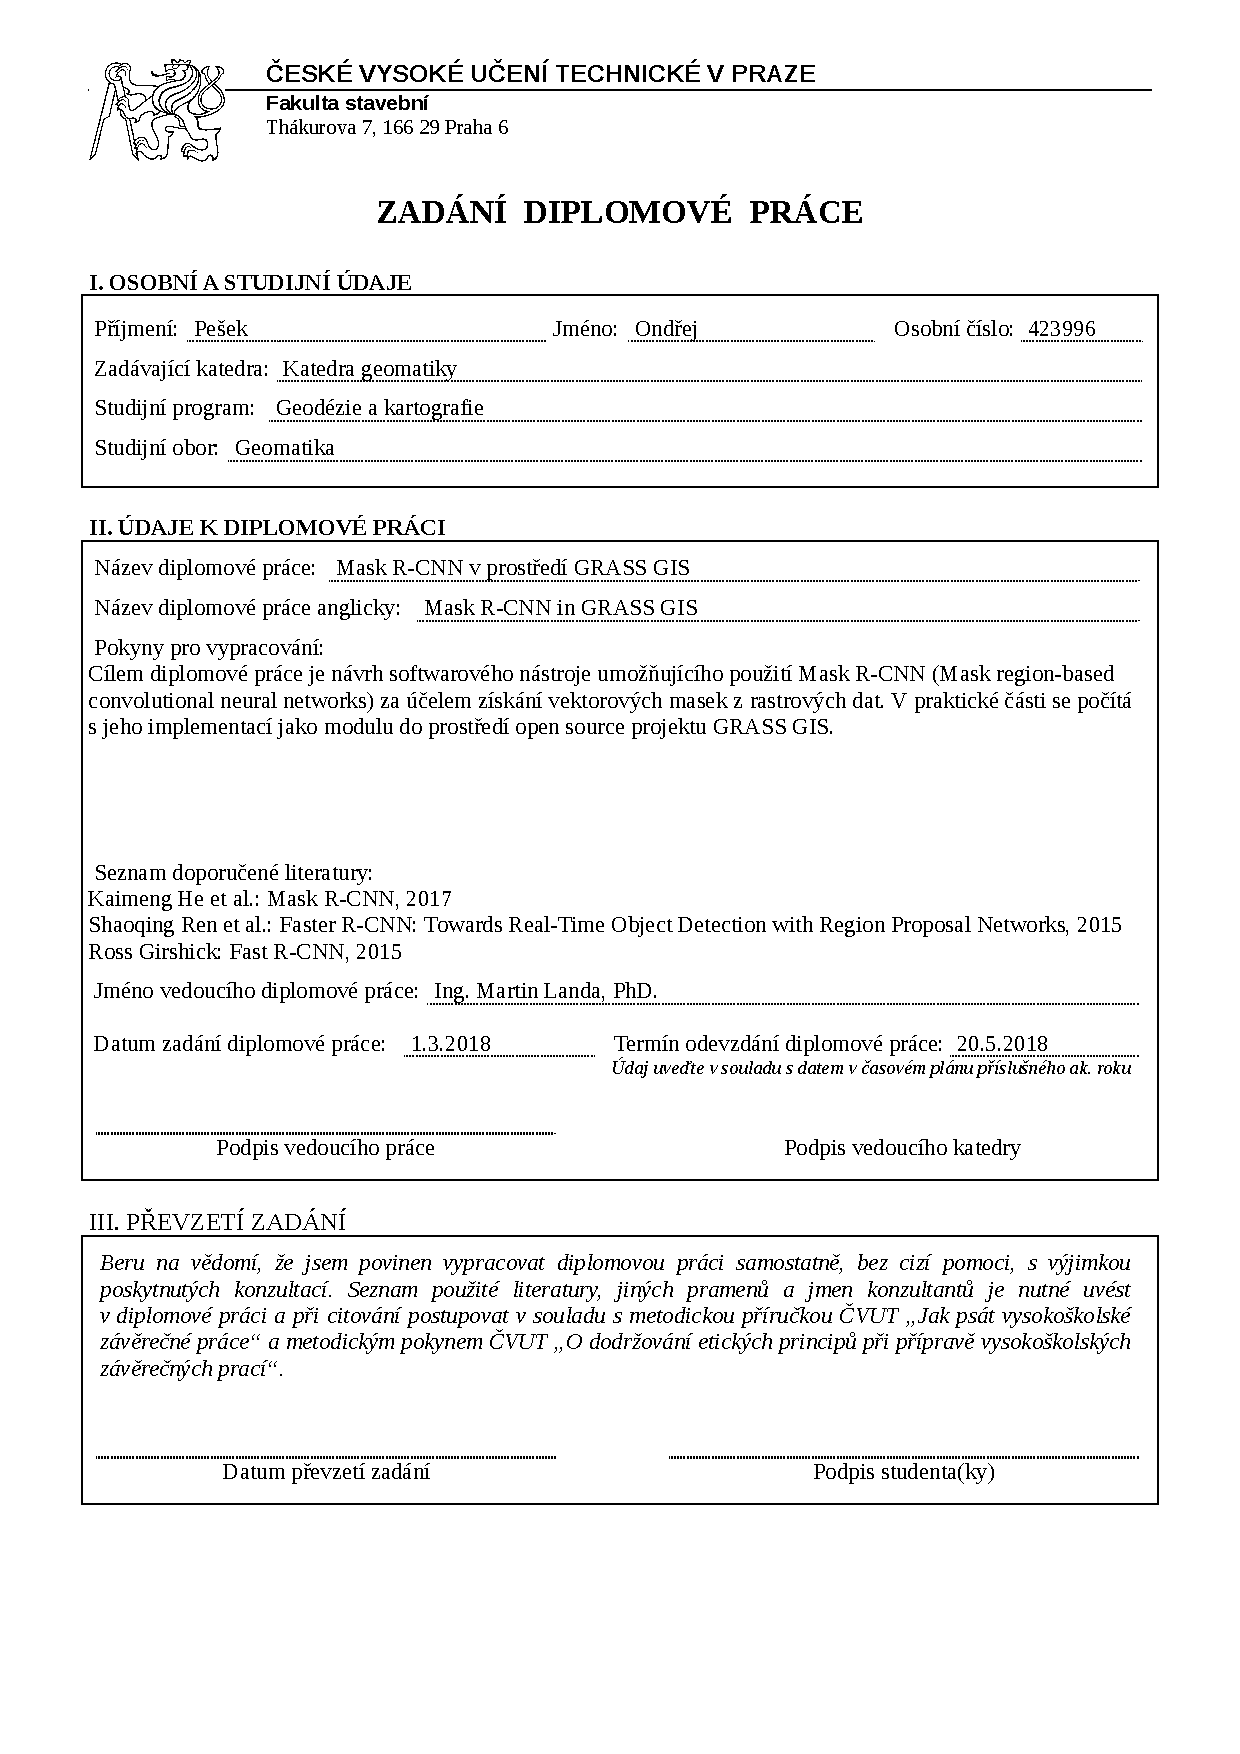
\includegraphics[scale=0.7]{./pictures/zadanidp.pdf}}%\sffamily\Huge\centering\ }%ZDE VLOŽIT LIST ZADÁNÍ}%
	%{\sffamily\centering Z~důvodu správného číslování stránek}

% vysázení stránky s abstraktem
\vytvorabstrakt

% vysázení prohlaseni o samostatnosti
\vytvorprohlaseni

% vysázení poděkování
\stranka{%nahore
       }{%uprostred
       }{%dole
       \sffamily
	\begin{flushleft}
		\large
		\MakeUppercase{Acknowledgement}
	\end{flushleft}
	\vspace{1em}
		%\noindent
	\par\hspace{2ex}
	{I would like to thank my parents for their support during my studies.
	Then I would like to thank Martin Landa, not only for supervising my thesis,
	but also for the initial impulse in direction to artificial neural networks
	and open source GIS generally. My thanks also belong to Margherita Di Leo for
	long initial discussions about the usage of neural networks in the field of
	GIS, to Moritz Lennert for testing and comments during the code sprint in
	Bonn, and to Luca Delucchi and Fondazione Edmund Mach for the willingness to
	exploit their time and resources to test modules.}
}

% vysázení obsahu
% \setcounter{tocdepth}{1}
\obsah

% vysázení seznamu obrázků
\seznamobrazku

% vysázení seznamu tabulek
% \seznamtabulek

% vysázení seznamu ukázek kódu
\cleardoublepage
\thispagestyle{empty}
 \lstlistoflistings
\newpage

% jednotlivé kapitoly
\chapter{Introduction}
\label{intro}

In the last years, the field of computer science is permanently shaken by one 
term: Artificial neural networks (\zk{ANN}s). Some people perceive it almost
as a magical formula. And even though \zk{ANN}s are not a spell able to solve
everything, they have wide applications. Their applications are in finance,
data mining, language recognition, computer vision and many more.

Another term that can be heard more and more is \textit{the information age}.
The~availability of computers and the growth of memory limits results in huge
amounts of data.

The huge amount of data is a fuel for \zk{ANN}s. One hundred years ago, an
artificial intelligence was a phantasmagoria of science-fiction writers. Fifty
years ago, it was an idea facing only derision. Twenty-five years ago, a design
doomed to failure due to a lack of training data. Twelve years ago, a bold idea
of few men. Five years ago, an earthquake in each branch of the field of
computer science.

The data availability and their opening in the field of geomatics, as well as
the~computer performance open doors for the usage of \zk{ANN}s in geographic
information systems (\zk{GIS}). Results of a special type of \zk{ANN}s called
convolutional neural networks (\zk{CNN}s) promises a lot in computer vision and
therefore also in \zk{GIS}, in tasks of detection and classification.

Chapter \ref{cnn} will briefly introduce the~theory behind \zk{CNN}s. In the
first part, the~history and the motivation behind them will be described. The
second part covers multiple types of layers used in \zk{CNN}s. Few pioneering
architectures will be covered.

Chapter \ref{image-ann} will introduce the term computer vision. Various tasks
of computer vision will be named and few breakthrough architectures not 
mentioned in the \zk{CNN} chapter will be described there. The research which 
concluded in the selection of Mask \zk{R-CNN} as the architecture for the 
implementation will be depicted in this chapter.

Chapter \ref{technologies} will introduce some of the most important 
technologies used during
the~above-mentioned implementation.

The implementation will be the topic of chapter \ref{implementation}. It will 
summarize the motivation behind the architecture choose and code decisions, and
then describe the~uppermost parts of the code. The practical part of the~thesis
is exactly this implementation.

\chapter{Convolutional neural networks}
\label{cnn}

% \setcounter{secnumdepth}{1}

Although it is assumed that the reader has sufficient prior knowledge of
%% ML: convolutional neural networks (CNN)
artificial neural networks and convolutional neural networks, this part briefly 
introduces convolutional neural networks, their layer types and few selected 
architectures. 

For better understanding of the topic, it is recommended to take a look at the 
holy book of deep learning, \cite{dl}.

\section{Introducing convolutional neural networks}
\label{understanding-cnn}

%% ML: prestoze je CNN uvedena v seznamu zkratek, tak bych ji
%% navrhoval v minulem odstavci zminit (viz predchozi poznamka)
If you try to find an introduction to \zk{CNN}s on the internet, you may bump 
into a common statement that \zk{CNN}s are neuroscience-based deep neural
networks using convolution and presuming the input is an image. It is not 
exact. 

Though images are the most common input, according to \cite{dl}, \zk{CNN}s 
presume the input has a grid-like topology; apart from the computer vision, 
other applications include  for example natural language processing (as in 
\cite{cnn-nlp}) or anything representable as a grid-like topology (audio 
waveform as 1-D grid, RGB images as multichannel 2-D, CT scan as 3-D, etc.). 

A paradox inexactness is the term \textit{convolution} as in mathematical 
meaning, many \zk{CNN}s implement cross-correlation instead of real convolution. 
Cross-correlation may be seen as convolution without a kernel flipping. The 
reader can get more mathematical insight about the difference and harmlessness 
of this change from \cite{dl}. 

It is true that \zk{CNN}s are based on a neuroscience. They are inspired by 
Nobel prize laureates Hubel and Wiesel's research on mammalian vision systems 
(firstly cats in \cite{hubel-cats1} and \cite{hubel-cats2}, later monkeys in 
\cite{hubel-monkeys}). Hubel and Wiesel found that some neurons (sorted in 
columns) strongly respond to specific edge-like patterns but just a 
bit to other patterns. 

The eye stimulus on the retina is transferred through the optic nerve and the 
lateral geniculate nucleus into the primary visual cortex (sometimes referred to 
as V1), a part of the visual cortex located in the posterior pole of the 
occipital lobe. The primary visual cortex is organized in a 2-D spatial map 
representing visual stimuli from the retina and contains two cell types, simple 
cells and complex cells. Simple cells purpose is to compute a linear function 
(although some counterarguments against the linearity have been raised, see 
\cite{simple-cells}) of the image in a spatially localized field, while complex 
cells operations are to some extent position and lighting invariant. 

\section{Layer types}
\label{layers}

While the common approach in image processing of classical \zk{ANN}s is to 
vectorize the input, \zk{CNN}s emulate the neuroscientific approach outlined in 
chapter \ref{understanding-cnn} using feature maps (each colour channel is a 
feature map). \zk{CNN}s profit from the fact that pixels in an image are ordered 
according to some structure. That allows neurons in layers to be connected just 
to certain region instead of heavily arduous fully-connected architecture. 

\zk{CNN}s consist from many layers with different functions. In the following, 
individual layer types are briefly described. 

\subsection{Convolutional layers}
\label{conv-layers}

The first layers through which is the input passed are convolutional layers. So, 
firstly, what is the convolution? 

In the geomatics field, we very often encounter the term \textit{kernel}. Kernel 
can be seen as a matrix (or a window) sliding across all the image pixels. The 
pixels contained in this window are a receptive field. As both the kernel and 
the receptive field are matrices of the same shape, in each position element-wise
multiplication is computed and outputted as an output matrix element. 
Because after such a filtering, the output matrix contains a 2-D activation map 
(a map where each position values say with which probability the requested 
feature is on that position in the original image), the output is called a 
\textit{feature map}. Kernels / filters are the subject of training. 

In case of stride 1 and without zero-padding, the feature map is naturally of 
shape $[original\_width - kernel\_width + 1] \times [original\_height - 
kernel\_height + 1]$. An example may be seen in figure \ref{fig:conv}. 

%% ML: reference/author?
\begin{figure}[H]
   \centering
	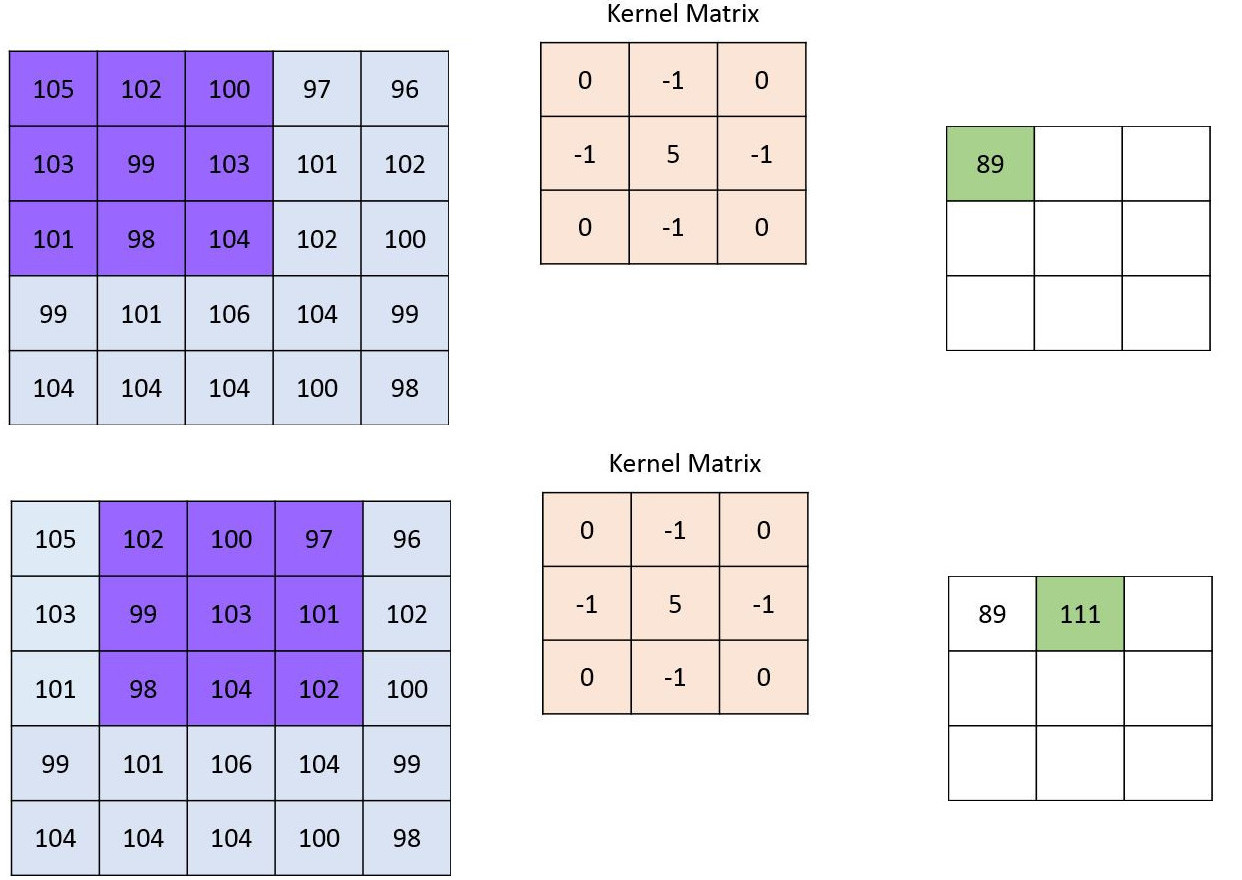
\includegraphics[width=.4\linewidth]{./pictures/conv.jpg}
	\caption[Kernel convolution]{Two steps of kernel convolution}
      \label{fig:conv}
\end{figure}

With convolution, we reduce both computational requirements and a threat of 
overfitting by using local connections (representing weights) between input and 
output. However, these connections are local only in two dimensions, in width 
and height of the input; these connections have to be full along the channels 
depth - e.g. in RGB images, the last dimension of connections is always 3. 
Different is it with the output; its third dimension (\textit{depth}) is 
determined by the number of neurons referencing the same spatial location, e.g. 
by the number of kernels we use. 

In chapter \ref{understanding-cnn}, translational invariance was mentioned. In 
convolutional layers, the first step to this invariance was achieved by another 
huge parameter reduction, by parameter sharing. Idea of parameter sharing raised 
from the premise that when one feature is useful in one location, it could be
%% ML: for for
useful also in another one. This simple presumption which works except for for 
example centered special structures allows sharing a set of parameters 
throughout the whole depth slice. 

Using the parameters from \cite{cnn-classification} as an example, assume that 
the feature map has size $55 \times 55 \times 96$ and we apply it to images of 
size $227 \times 227 \times 3$\footnote{The paper claims that the images were of 
size $224 \times 224 \times 3$, but it is assumpted that it was either a typo or 
authors forgot to mention a zero-padding} using kernels of size $11 \times 11 
\times 3$. Sharing parameters within a depth slice, we can reduce the parameter 
amount from $55 * 55 * 96 * (11 * 11 * 3 + 1)$ to $96 * (11 * 11 * 3 + 96)$ (1 
and 96 are biases), it means from more than 105 millions to less than 35 
thousands. Speaking only about the first layer. I believe that this example said 
it all. 

An inquiring reader may raise a question: In the chapter name, there is a 
plural. What happens in deeper layers? 

Their input is the previous layer output. Output of the first layer is the 
feature map of the lowest-level features. As was already mentioned, each neuron 
of the next layer is connected with some local neighbourhood and with everything 
along the third dimension; and because the third dimension of the output is 
formed by stack of filters / kernels of the first layer, each second layer 
neuron is connected to all detected features in some location and its 
neighbourhood. The result? Output feature map from the second layer contains 
higher-level features (simple combinations of the low-level ones, like triangles 
or squares; combinations of some edges, curves, etc.). The next layer 
will output again higher-level features and in the end, we may have very 
specific features like cars, reflective heliports or art deco swimming pools. 
This principle is illustrated in figure \ref{fig:deconvnet} using a 
deconvolutional network, a technique described in chapter \ref{zfnet}.

\subsection{ReLU layers}
\label{relu-layers}

Since the real data we are using to train our \zk{CNN}s are mostly non-linear, 
it is useful to introduce some non-linearity into the network. In the past, 
functions like hyperbolic tangent or sigmoid were used, but Rectified Linear 
Unit (\zk{ReLU}) has been found to be trained faster and mitigate the vanishing 
gradient problem (problem of slow training of low layers due to the exponential 
decrease of the gradient). 

\zk{ReLU} output is defined by a function:

$f(x) = max(0, x)$

%% ML: ... to of ...
After applying the \zk{ReLU} function to of the input values, we have a feature 
map where all negative values of the input were changed to zero. This output is 
called \textit{rectified feature map}. 

\subsection{Pooling layers}
\label{pooling}

Even though the input size reduction might already be included in convolutional 
layers, it is very common to include another layers with this purpose. Because 
of this purpose, they are called \textit{pooling layers} or \textit{subsampling 
layers} (they can do both downsampling or upsampling). 

Pooling layers work again with a kernel. But this time, the stride is bigger 
than one which is quite uncommon for convolutional layers. It means that when we 
use a pooling layer with kernel of size 2$\times$2 and stride 2, the output will 
be half in first two dimensions (the third one is preserved). One pooling like 
this reduces parameters by 75 percent. 

Aside from the parameter reduction, there are two more positive effects. Because 
of the detail mute, it reduces a threat of overfitting and it also strengthens 
the shift invariance. The advantage of pooling layers is also the fact that they 
do not introduce no new parameters to the network. 

The function for the kernel can vary, but the most-used one is 
max-pooling\footnote{Choosing the biggest value from those overlaid by the 
kernel.} having the advantage that it does not matter where in the region was 
the value detected. Other customary approaches apply average (compared with 
max-pooling in \cite{avg-pooling}), $L2$ \cite{l2-pooling} or Stochastic pooling 
\cite{stoch-pooling}. Also used kernel size and stride vary, the most common 
ones are 2$\times$2 with stride 2 and 3$\times$3 with stride 2. 

Also, architectures without pooling layers are not so uncommon today. One 
research on this approach can be seen in \cite{all-conv-net}. It introduces an 
architecture called \textit{all convolutional net} where the subsampling may be 
done by increasing the stride and compares it with other approaches. 

\subsection{Normalization layers}
\label{norm-layers}

Besides neural exhibition, neural inhibition is also found in the human brain. 
These doors of perception stay half-closed and filter or inhibit human 
receptions.

Normalization layers can be seen as an attempt to imitate this structure, but 
there are more reasons for these layers in deep learning. As was written above, 
input for higher (deeper) layer is the output of lower level. It means that the 
highest (deepest) layer input is dependent on the first layer output. Because 
functions of layers are changed each training step, a small change of the first 
layer output may have huge effect on the last layer input and therefore also on 
the last layer output, which may lead to completely wrong behaviour of deeper 
layers. This problem is called a \textit{covariate shift} or, following 
terminology from \cite{batch-norm}, an \textit{internal covariate shift}. 

This change in the distribution can be to some extent reduced by using a small 
learning rate and right initialization of the network. Because small learning 
rate radically extends the training time, other solutions were needed. 
Normalization layers. 

One of the most widely used approaches is called \textit{batch normalization} 
\cite{batch-norm}. In \zk{CNN}s, it is common to use batches (or mini-batches) 
of training examples instead of one-at-a-time as the computation parallelism 
saves time. Batch normalization computes a mean and variance over a batch using 
the distribution of the summed neuron input and whiten\footnote{Set means equal 
to zero and variances unit; idea proposed in \cite{tricks}.} it for each 
training batch. According to \cite{batch-norm}, it reduced the number of 
training steps 14 times allowing the user to use much higher learning rate and 
being less careful about initialization.

Another types of normalization layers include local response normalization or 
$L2$ normalization.

\subsection{Fully connected layers}
\label{fc-layers}

As their name prompts, fully connected (\zk{FC}) layers are layers where each 
neuron in a layer is connected to each neuron of the previous layer. Their 
activations can be seen simply as a matrix multiplication enhanced by a bias.  

The purpose of \zk{FC} layers is to take the high-level feature map as an input 
and return a classification vector as an output. Each value in the output refers 
to one class occurrence, e.g. the length of the output vector is $n$ where $n$ 
is the number of classes. \zk{FC} layers are not so hard to train to use 
non-linear combinations of features in input which is widely used whereas the 
combinations of high-level features are the things we are looking for. For 
example, if we are looking for a platypus, the last layer output will have high 
values in the neurons that represent things like a duck-like snout, four legs, 
flat tail or a calcaneus spur; if we are looking for a jelly, we will most 
probably not be interested in any of these features. 

Using popular \textit{softmax} classifier\footnote{Softmax transforms a vector 
of real-valued values to a vector of values between zero and one that sum to 
one.}, the output is a vector of probabilities representing each class. Other 
classifiers like \zk{SVM} can also be used. 

Fully connected layers are sometimes referred to also as \textit{dense layers}.

\section{Architectures of convolutional neural networks}
\label{cnn-architectures}

It is generally resolved\footnote{Roots of \zk{CNN}s are in the end of eighties, 
but the breakthrough came in nineties.} that the history of successful \zk{CNN}s 
started in 1998 when Yann LeCun and his team published the paper Gradient-Based 
Learning Applied to Document Recognition \cite{lenet5}. Although it is just 
twenty years, \zk{CNN}s have made tremendous progress. During this period, a 
plenty of various architectures was proposed, more or less successful.

Because some background of the \zk{CNN} architectures evolution could help in 
understanding \zk{CNN} fundamentals and deepens the insight into research and 
decisions made for this thesis, few of the most influential architectures will be 
mentioned in the following chapters.

In this chapter, ImageNet Large Scale Visual Recognition Challenge (\zk{ILSVRC}) 
will be mentioned several times as it is something like a fuel for computer 
vision progress with which are \zk{CNN}s inseparably connected. For the topic of 
this thesis, it should be enough to say that \zk{ILSVRC} is a competition in 
visual recognition including many diverse tasks, for more informations and 
results take a look into \cite{ILSVRC} which was used also during writing this 
chapter.

\subsection{LeNet-5} %
\label{lenet}

Nobody would argue that the fundamental architecture is the one from the paper 
Gradient-Based Learning Applied to Document Recognition mentioned above, the one 
called LeNet-5. It was proposed in \cite{lenet5} and due to the lack of GPU and 
insufficience of CPUs, its convolutional, computationally economical approach 
ensured the architecture a huge success and usage for example in character 
recognition (reading zip codes, checks). 

In figure \ref{fig:lenet}, we can see the architecture of LeNet-5. It contains 
many features mentioned in chapter \ref{layers}. It consists of convolutional, 
pooling (subsampling) and \zk{FC} layers and it also introduced the 
non-linearity into the network using hyperbolic tangent or sigmoids. Its two 
convolutional layers (C1 and C3) apply $5 \times 5$ convolutional filters with 
stride $1$ and its two pooling layers (S2 and S4) apply $2 \times 2$ 
average-based filters with stride $2$. The architecture is finished with two 
\zk{FC} layers; one is needed to learn the non-linear combinations of high-level 
features, the other one to classify the results\footnote{Gaussian connections 
are used here instead of softmax mentioned in \ref{fc-layers}. They are based on 
Euclidean Radial Basis Function and described in \cite{lenet5}.}.

\begin{figure}[H]
   \centering
	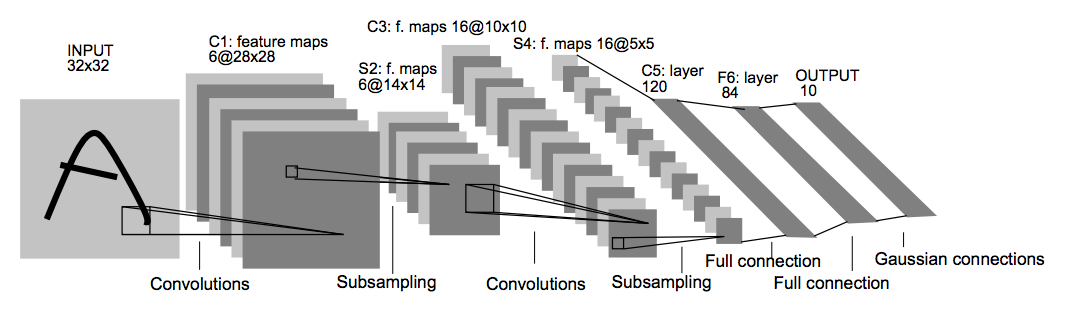
\includegraphics[width=\linewidth]{./pictures/lenet.png}
	\caption[LeNet-5 architecture]{LeNet-5 architecture schema, source: 
\cite{lenet5}}
      \label{fig:lenet}
\end{figure}

LeNet-5 made the first important step for \zk{CNN}s and a big step for 
\zk{ANN}-based computer vision generally. It explained that taking an input as 
individual values - besides its speed and computation problems - does not use 
the advantage of spatial correlations within the input. 

%\subsection{Dan Ciresan Net}
%\label{ciresan}

% first with GPU
% 2010
% if uncommented, change begining of AlexNet

\subsection{AlexNet} %
\label{alexnet}

As was mentioned, LeNet-5 became very successful first step. Nevertheless, until 
2010s, development of \zk{CNN}s was out of the main spotlight. Although there 
were few important events like Dan Ciresan using GPU neural nets in 2010, the 
main one happened in 2012, when Alex Krizhevsky came with something like a 
deeper version of LeNet in \cite{cnn-classification} and called it AlexNet. That 
year, AlexNet won the \zk{ILSVRC}\footnote{AlexNet won it by a great margin with 
top 5 error of 16.4 \% compared to the second place with 26 \%.}.

Krizhevsky benefited from years of progress bringing more computing power and 
more data to be trained on. This well-timed entree allowed him to use a deep 
architecture containing about sixty millions parameters, \zk{ReLU} layers, 
overlapping max pooling and dropout\footnote{A technique used to prevent 
overfitting proposed in \cite{dropout}. Dropout selectively ignore individual 
neurons during training.}. AlexNet also included a stack of convolutional layers 
instead of previous approach, where each convolutional layer was followed by a 
pooling layer. 

The computation was done on GPU (NVIDIA GTX 580) which allowed him to use larger 
datasets consisting of more and larger images as well as fastened the training. 
The separate GPU approach is indicated in figure \ref{fig:alexnet} by upper and 
lower part of the image as two different GPU processes; it can be seen that the 
interaction between two GPUs happens only at certain layers. 

\begin{figure}[H]
   \centering
	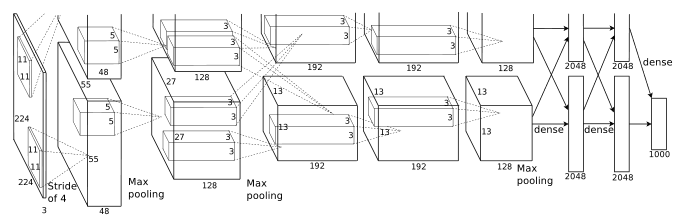
\includegraphics[width=\linewidth]{./pictures/alexnet.png}
	\caption[AlexNet architecture]{AlexNet architecture schema, source: 
\cite{cnn-classification}}
      \label{fig:alexnet}
\end{figure}

If LeNet-5 represents the first step of \zk{CNN}s, AlexNet is the first 
marathon. After its success, \zk{CNN}s became the bleeding edge in both deep 
learning and computer vision. 

% CS231n about zero-padding

\subsection{ZF Net}
\label{zfnet}

After the success of AlexNet, the number of \zk{CNN}s competing in the ImageNet 
Large Scale Visual Recognition Challenge (\zk{ILSVRC}) noticeably increased. 
Matthew Zeiler and Rob Fergus built an architecture called ZF Net and won the 
\zk{ILSVRC} 2013 with top 5 error rating of 11.2 \%. 

ZF Net architecture was based on AlexNet and described in \cite{zf-net}. Because 
it was believed that the $11 \times 11$ filtering in the first layer of AlexNet 
skipped too much information, it was replaced with a filter of size $7 \times 7$ 
with a decreased stride. Besides the parameter tweaking, the size of the middle 
convolutional layers expanded and the cross-entropy loss function was used as 
well as stochastic gradient descent with a mini-batch size of 128. The 
architecture can be seen in figure \ref{fig:zf-net}.

\begin{figure}[H]
   \centering
	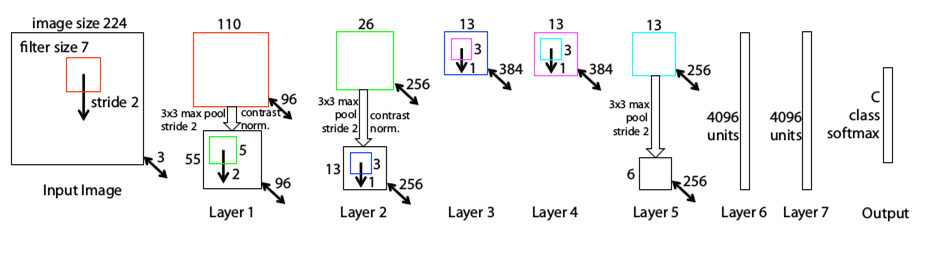
\includegraphics[width=\linewidth]{./pictures/zf-net.png}
	\caption[ZF Net architecture]{ZF Net architecture schema, source: 
\cite{zf-net}}
      \label{fig:zf-net}
\end{figure}

An important feature was introducing a technique mapping features from feature 
maps back to pixels, due to its character this technique is called a 
\textit{deconvolutional network}. During the forward pass, activations are 
computed at each level of \zk{CNN}s; when we want to observe a certain feature 
of a certain layer, we pass it back through the preceding layers. In this back 
pass, operations are in another direction (pooling is changed to unpooling, 
downsampling to upsampling etc.) until the input layer is reached. It gives the 
user an idea of what kinds of structures are recognized in the certain feature 
map. A visualization of 5 layers illustrating the way from low-level features 
like edges or colours to high-level features like dog faces or flowers can be 
seen in figure \ref{fig:deconvnet}.

\begin{figure}[H]
   \centering
	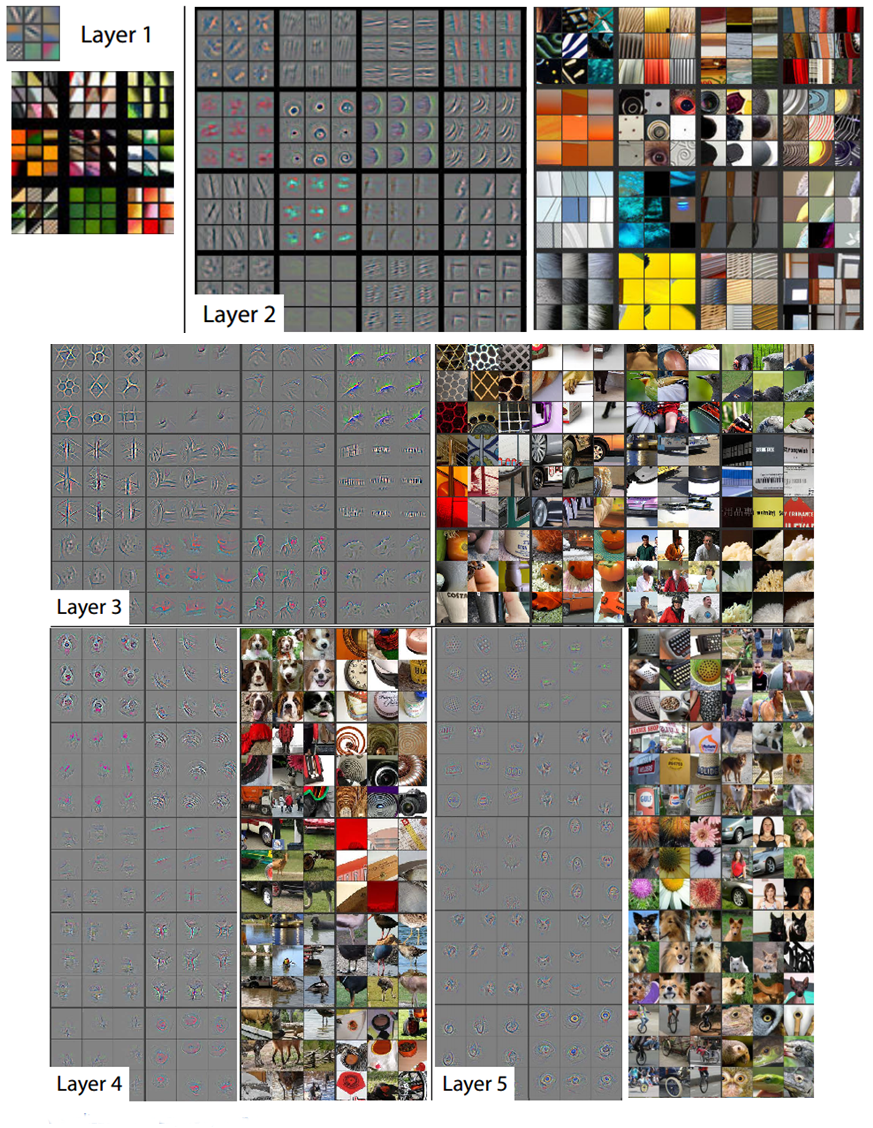
\includegraphics[width=\linewidth]{./pictures/deconvnet.png}
	\caption[Deconvolutional network]{Visualization of 5 feature maps through 
deconvolutional networks, source: \cite{zf-net}}
      \label{fig:deconvnet}
\end{figure}

Thanks to its modifications, it was enough to train ZF Net on only 1.3 million 
images instead of 15 million images used with AlexNet. However, the training 
took 12 days instead of 5 or 6 and was stopped after 70 epochs. The training ran 
on a single GPU.

However, in \cite{zf-net}, Zeiler and Fergus did more than just bring new 
architecture. They summarized why the time of \zk{CNN}s had just come and tried 
to deepen the general knowledge behind these models, where especially the 
deconvolution visualization of feature maps can be called a missionary work.

\subsection{VGG Net}
\label{vgg}

\zk{ILSVRC} 2014 brought new interesting architectures. Although VGG Net, an 
architecture proposed by Visual geometry group of the University of Oxford in 
\cite{vgg}, was not the winning architecture, it reached the error rate 7.3 \% 
even with its \textit{simplicity-in-the-first-place} architecture.

Authors experimented with different architectures with number of layers between 
11 and 19 (see figure \ref{fig:vgg} for their parameters) and chose 16-layer 
architecture homogenously using only $3 \times 3$ filters with stride and zero 
padding of size 1 to preserve the spatial resolution after convolution 
interleaved with maxpooling layers with stride 2. They found that when we use 
multiple convolutional layers with smaller kernels in a row, it emulates the 
effect of larger kernels while still retaining advantages of smaller kernels; it 
means that 3 layers with kernel $3 \times 3$ emulate the effect of 1 layer with 
kernel $7 \times 7$, decrease the number of parameters and allows the user to 
implement three ReLU layers instead of one, exactly the advantage VGG Net used. 
It has to be said that the number of parameters was still enormous reaching 
almost 140 millions and in the following architectures, this problem caused by 
\zk{FC} layers had to be solved to reduce the time consumption.

VGG Net also enlarges the number of filters after each maxpool layer as can be 
seen in figure \ref{fig:vgg}; the idea of decreasing spatial dimensions but 
increasing the third (depth) dimension was shown to be very important as well as 
the depth (number of layers) of the network. During the mini-batch gradient 
descent based training, a scale jittering was used for the data augmentation to 
train the model to recognize objects at different scales. The training took two 
to three weeks depending on the architecture and was carried out by 4 NVIDIA 
Titan Black GPUs.

\begin{figure}[H]
   \centering
	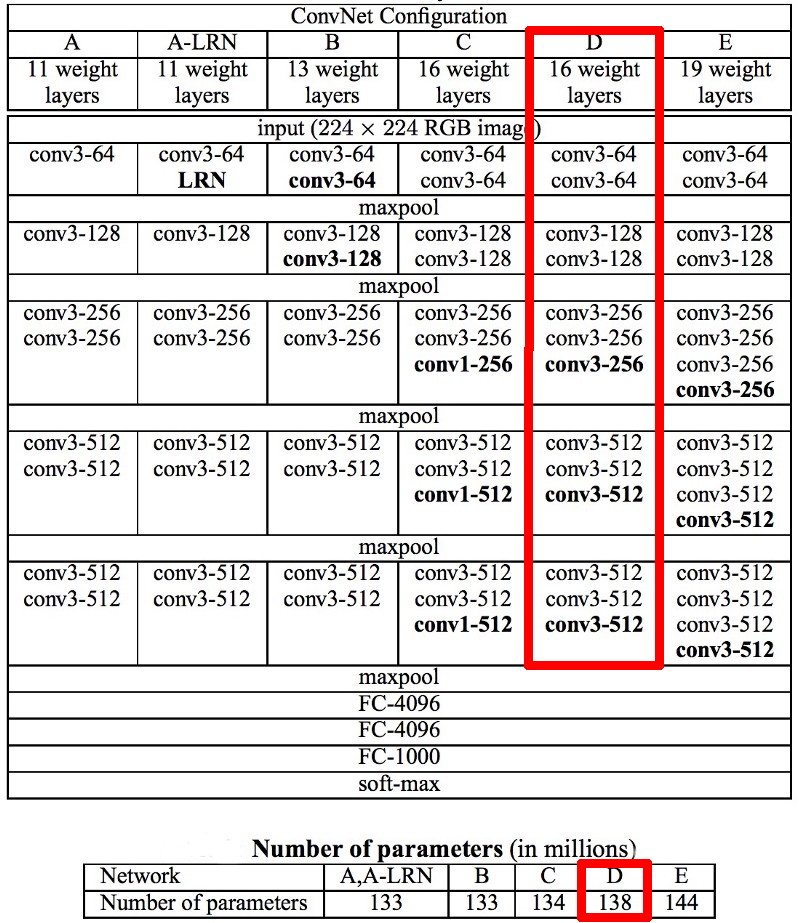
\includegraphics[width=0.8\linewidth]{./pictures/vgg-net.png}
	\caption[VGG Net networks]{Different architectures of VGG Nets and the chosen 
one, source: \cite{vgg}}
      \label{fig:vgg}
\end{figure}

% localization regression pp 10 of {vgg}
% Caffe

% \subsection{Network-in-network}
% \label{nin}

% 1x1 convolutions
% if uncommented, change footnote in googlenet

\subsection{GoogLeNet}
\label{googlenet}

And now for something completely different. Authors of GoogLeNet, the winning 
architecture of \zk{ILSVRC} 2014 with a top 5 error rate of 6.7 \%, proposed in 
\cite{googlenet} another approach, instead of at the architecture simplicity 
aiming at the computational simplicity.

\begin{figure}[H]
   \centering
	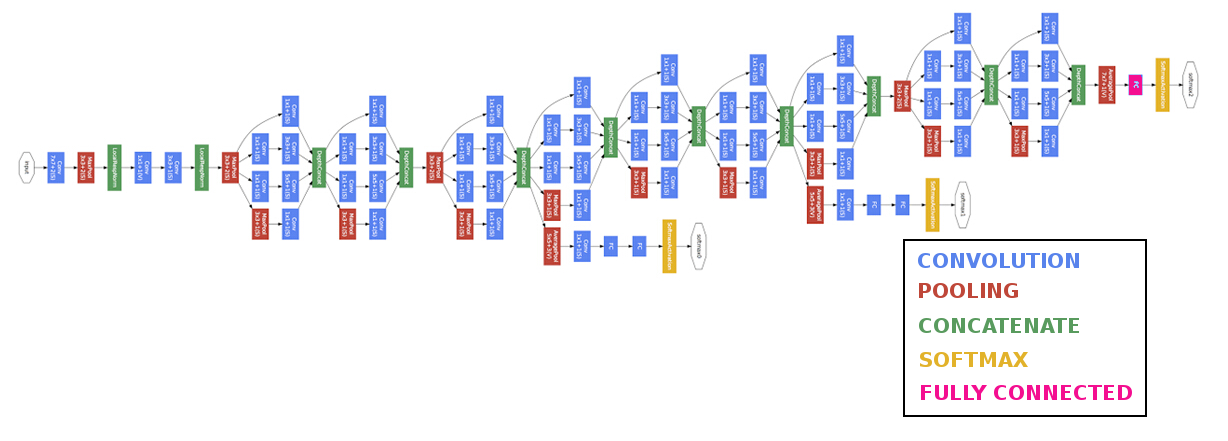
\includegraphics[width=\linewidth]{./pictures/googlenet.png}
	\caption[GoogLeNet networks]{GoogLeNet network schema, source: 
\cite{googlenet}}
      \label{fig:googlenet}
\end{figure}

In figure \ref{fig:googlenet}, we can see parallel blocks. Authors found that 
the sequential queue of layers increases a computational and memory cost a lot,
%% ML: naivni, ale pekne
so they proposed a module called \textit{Inception}. The naïve idea behind the 
Inception module is illustrated in figure \ref{fig:inception-naive} and is quite 
simple: Why should we stack the layers in a sequence, when we can perform them 
in a parallel? Though the idea behind was not bad, this naïve version ended in 
an enormous depth (size of the third dimension) of the output after the 
concatenation into a single vector.

\begin{figure}[H]
   \centering
	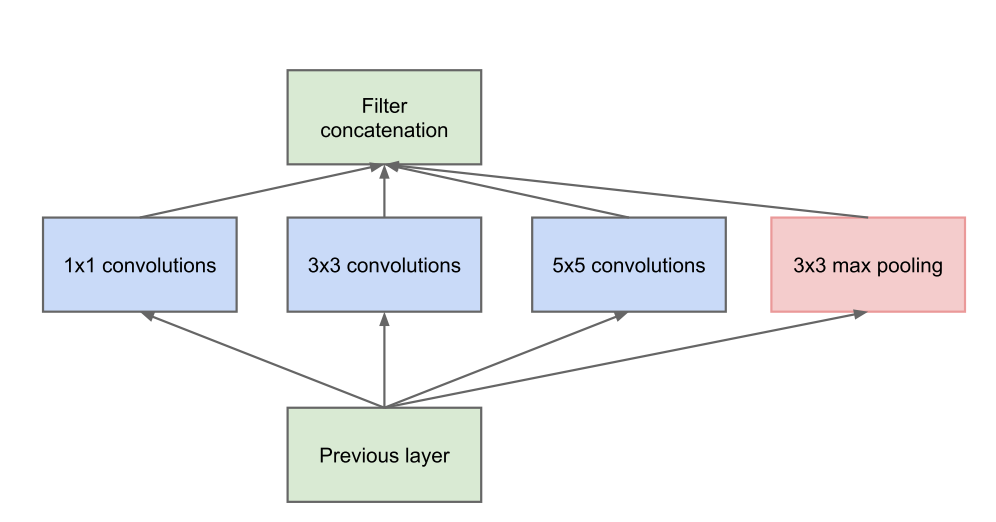
\includegraphics[width=0.8\linewidth]{./pictures/inception-naive.png}
	\caption[Inception module, naïve idea]{Naïve idea of Inception module, source: 
\cite{googlenet}}
      \label{fig:inception-naive}
\end{figure}

As can be seen in figure \ref{fig:inception-full}, authors solved the depth 
problem by adding $1 \times 1$ convolutional layers, sometimes referred to as 
\textit{network in network}\footnote{The alias of this approach was derived from 
the architecture called Network-in-network proposed in \cite{nin} and presenting 
the advantages of $1 \times 1$ convolutions.}. Usage of 10 $1 \times 1$ filters 
outputs a volume with two dimensions equal to the input dimensions and the third 
one equal to 10. The depth of input for bigger kernels is thus \textit{pooled} 
to the defined size, while allowing also to use one more ReLU layer after the $1 
\times 1$ convolution. This process is sometimes called a \textit{bottleneck} 
(likewise the $1 \times 1$ layer is sometimes called a \textit{bottleneck 
layer}).

\begin{figure}[H]
   \centering
	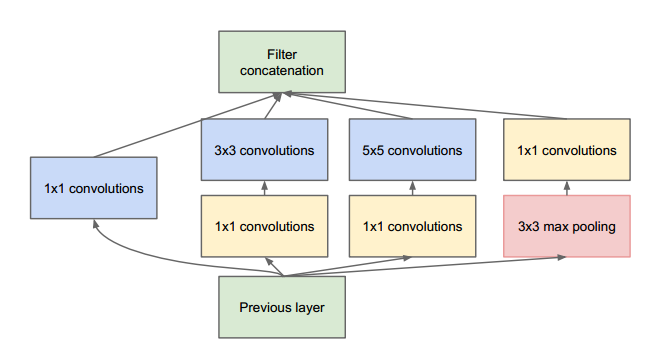
\includegraphics[width=0.8\linewidth]{./pictures/inception-full.png}
	\caption[Inception module, full]{Inception module with dimensionality 
reduction, source: \cite{googlenet}}
      \label{fig:inception-full}
\end{figure}

The parallelized architecture used over 100 layers while the real depth of the 
full network was just a fraction of this number and it used only 7 Inception 
modules. Authors also get rid of unnecessary \zk{FC} layers and instead used an 
average pooling which concluded in twelve times fewer parameters than AlexNet. 
Their architecture also decreased the threat of overfitting. In 
\cite{googlenet}, authors claimed that the network was trained \textit{using few 
high-end GPUs within a week}.

Time from time, updated versions are published. Interested readers may try to 
find architectures like Inception V2, Inception V3 and higher.

\begin{figure}[H]
   \centering
	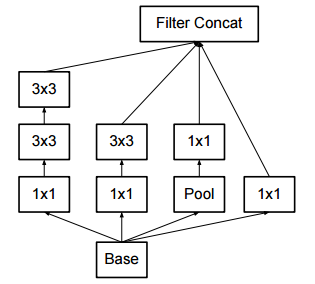
\includegraphics[width=0.3\linewidth]{./pictures/inception-v2.png}
	\caption[Inception V2]{Inception V2 used the idea described already in chapter 
\ref{vgg} about replacing $5 \times 5$ convolution with two $3 \times 3$ 
convolutions, source: \cite{inception-v2}}
      \label{fig:inception-v2}
\end{figure}

%\subsection{Inception V3}
%\label{inception}

\subsection{ResNet}
\label{resnet}

In the above-described architectures, a trend of going deeper can be noticed. 
Microsoft Research team noticed it too and in \cite{resnet}, they proposed much 
deeper architecture than previous ones. This architecture was called ResNet, 
contained 152 layers and won \zk{ILSVRC} 2015 with an error rate of 3.6 \% 
beating even humans with their error rate of circa 5 -- 10 \%.

Although the depth was quite revolutionary, it was not the most innovative thing 
of ResNet. Neither was the usage of batch normalization as described in 
\cite{batch-norm} after each convolutional layer. The most innovative thing of 
ResNet was a structure called a \textit{residual block}. In 2011, Pierre 
Sermanet and Yann LeCun proposed in \cite{bypass} a notion to \textit{bypass} a 
layer. ResNet used this design with a richer mind and as can be seen in figure 
\ref{fig:res-block}, they bypassed two layers.

\begin{figure}[H]
   \centering
	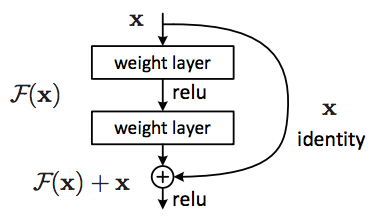
\includegraphics[width=0.4\linewidth]{./pictures/residual-block.png}
	\caption[Residual block]{A residual block schema, source: \cite{resnet}}
      \label{fig:res-block}
\end{figure}

Bypassing two layers (a term \textit{skip connections} is not uncommon) gives 
much better improvements than the single layer bypass. But what exactly happens 
during the bypass? In traditional \zk{CNN}s, only the $F(x)$ is computed. It 
means that the next layer does not have the real connection to the original 
input, but only to this transformed output, $F(x)$. When we bypass the block 
input $x$ after 2 layers, we can add it to $F(x)$ which represents a change this 
time. By the addition, we get a mildly altered representation of the input. 
Authors of ResNet declared that it is easier to optimize this referenced mapping 
instead of the unreferenced one. Another advantage is that with addition 
operations, the backward propagated gradients will flow easier through the 
structure. Because the mapping was referenced using residuums, it is sometimes 
referred to as a \textit{residual mapping}.

Authors experimented with diverse depths of the architecture counting 18, 34, 
50, 101 and 152 layers. During these experiments, authors found a problem in 
number of parameters in deeper architectures. However, they found a solution by 
following the design of bottleneck layers described in chapter \ref{googlenet}: 
They redesigned the residual block into a bottleneck block. This block reduced 
the number of features usually to one quarter by using $1 \times 1$ convolutions 
and was implemented into ResNet-50 and higher.

\begin{figure}[H]
   \centering
	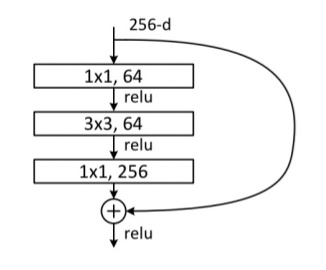
\includegraphics[width=0.4\linewidth]{./pictures/bottleneck-block.jpg}
	\caption[Bottleneck block]{A bottleneck block schema, source: \cite{resnet}}
      \label{fig:bottleneck-block}
\end{figure}

Mentioned experiments contained one more interesting event. A creation of a real 
monster, a 1202-layer network. Surprisingly, this network got a lower accuracy 
during tests. Authors argued that this is because of overfitting.

8 GPUs were used for the training of ResNet-152 and the process took something 
between two and three weeks.

The continuation of ResNet can be found for instance in an architecture called 
ResNeXt. Saining Xie and his team proposed ResNeXt in \cite{resnext} and it 
combines ResNet with modularized parallel pathways similar to those described in 
chapter \ref{googlenet}.

% \subsection{SqueezeNet}
% \label{squeezenet}

% \subsection{ENet}
% \label{enet}

\chapter{CNNs for computer vision}
\label{image-ann}

A paper Visualizing and Understanding Convolutional Networks by Matthew D. Zeiler and Robert Fergus \cite{zf-net} started with two sentences: \textit{Large Convolutional Network models have recently demonstrated impressive classification performance on the ImageNet benchmark. However there is no clear understanding of why they perform so well, or how they might be improved.}

I tried to disperse such clouds a bit in the previous chapter, but now I would like to focus on another undertone connected with those statements. On their applications in the computer vision.

Almost everything mentioned in chapter \ref{cnn} was already tied to the computer vision. The following text will briefly describe the field of computer vision itself and then introduce few tasks in that field connected with the topic of the thesis. In each task, few \zk{CNN} models will be mentioned. This text structure was chosen also to depict the models evolution concluding in the one selected for the practical part of this thesis - an implementation into GRASS GIS.

% different sizes

\section{Understanding computer vision}
\label{computer-vision}

When you see a group photo, you can easily count the number of people in the photo, you can say whether they are smiling or not, whether they are happy, sad, angry, you can even guess whether they are one family, a bunch of friends, colleagues or just random people passing by. You can do all of that in a fraction of a second without any effort. The computer vision is supposed to be a computer-aided version of this human cognition. Or in a fancier way, from \cite{opencv}: \textit{Computer vision is the transformation of data from a still or video camera into either a decision or a new representation.} The new representation might be for instance a colour shift, the decision an answer on a question like \textit{Is there any football field in the picture?}

However, the problem is that the claim that it is easy for humans does not mean that it is easy also for computers. As is generally known and was indicated in chapter \ref{understanding-cnn}, the human brain is an extremely complex tool. The other thing is that a computer receives a visual impulse (image) in other way as is illustrated in figure \ref{fig:mirror}. Where human sees a side mirror, a computer sees a grid of numbers. And this grid may be completely different when the daytime, viewpoint, brightness, background or scale changes.

\begin{figure}[H]
   \centering
	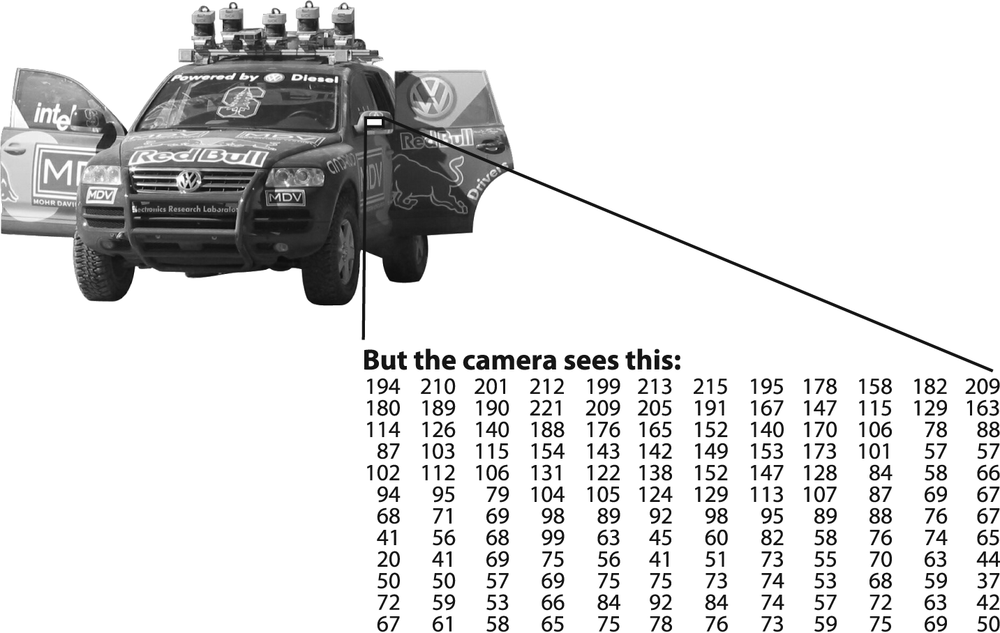
\includegraphics[width=.8\linewidth]{./pictures/comp-vision.png}
	\caption[Human and computer cognition]{The difference between human and computer cognition, source: \cite{opencv}}
      \label{fig:mirror}
\end{figure}

The task may be something like \textit{Is there any side mirror in the picture?} This kind of tasks can be seen in the field of computer vision daily and can be extremely difficult to solve in the computer way. Although the input may include some metadata, it still has to be solved in a strict mathematical way. And because our goal is to make our computer vision system \textit{perceive like a human}, it looks like the right place for \zk{CNN}s.

Although we will focus only on classification and connected tasks like detection and segmentation, there are many more applications of the computer vision. To name a few: Autonomous cars, face recognition, fingerprint recognition, motion capture, biometrics and remote sensing.

To get a better view into the field of computer vision, it is recommended to read a richer source like \cite{comp-vision} and \cite{opencv} to get some practice.

\section{Classification}
\label{classification}

\section{Classification with localization}
\label{classification-localization}

\section{Object detection}
\label{object-detection}

\subsection{R-CNN}
\label{r-cnn}

% R-CNN, Fast, Faster
% Single-Shot MultiBox Detector (SSD) You Only Look Once (YOLO)

\section{Semantic segmentation}
\label{semantic-segmentation}

% CNN

\section{Instance segmentation}
\label{instance-segmentation}

% Mask R-CNN

% \section{Content-based Image Retrieval}
\chapter{Used technologies}
\label{technologies}

\section{GRASS GIS}
\label{grass}

\section{Python}
\label{python}

\section{TensorFlow}
\label{tf}

\section{Keras}
\label{keras}
\chapter{Implementation}
\label{implementation}

In the field of \zk{GIS}, users are dealing with a huge amount of satellite photos. Though 
there are many algorithms for an automated classification, \zk{ANN}s are a 
promising child which is just growing up and hogging the limelight. However, the 
younger sibling of \zk{ANN}s is even more promising. The sibling is called 
\zk{CNN}s.

\zk{CNN}s for image processing are very strong in an object detection. The 
object detection in aerial photos could be very useful for example for detecting 
sick trees in an ortophoto of a forest or for a vehicle detection (airplane, 
ship, car, etc.). It means elements that can be represented as points. But what 
about searching for forests? Searching for lakes? Rivers? Oil spills? Do we 
really want to represent them in \zk{GIS} as points in their center of mass?

It seems that better representation is in polygons (or lines). But representing 
a detection bounding box as a polygon square does not seem like the right way. 
So there are two possible ways - semantic segmentation and instance 
segmentation. Three arguments were raised and discussed in behalf of instance 
segmentation:
\begin{itemize}
	\item The instance differentiation could be very useful in some tasks.
	\item It is easier to create masks only for requested objects.
	\item If each pixel in a raster input will be assigned to a class, we got \textit{semantic segmentation}.
\end{itemize}

When works on this implementation started, the paper on Mask R-CNN was just 
recently published (\cite{mask-rcnn}, March 2017). With its approach, it was a 
kind of bleeding edge. However, its results spoke for themselves and within a 
year of its publication, it was implemented in few projects following the 
success of the original paper. Few followers also appeared (for example 
\cite{masklab}) and it could be interesting to examine them deeper from a 
geomatic point of view.

For the implementation to GRASS GIS, the Python language was chosen. There are 
few reasons for this decision:
\begin{itemize}
	\item Although some GRASS GIS modules are written in C and C++, many of them are written in Python.
	\item Python allows me to use libraries such as TensorFlow\footnote{\url{https://www.tensorflow.org/}} and Keras\footnote{\url{https://keras.io/}}, both very useful and widely used in the field of deep learning. 
\end{itemize}

Mask \zk{R-CNN} tools created for the practical part of the thesis consist of 
two modules. \verb|ann.maskrcnn.train| allows user to train a Mask R-CNN model 
on his own dataset, \verb|ann.maskrcnn.detect| allows him to use that model to 
detect features in georeferenced files. Both modules are licensed under GNU \zk{GPL} 2 license.

Along with these modules, a library of Mask \zk{R-CNN} tools was prepared. This 
library was heavily based on a Python implementation of Mask \zk{R-CNN} written 
by Waleed Abdulla from Matterport, 
Inc.\footnote{\url{https://matterport.com/about/}}  Matterport, Inc. published 
their implementation under the MIT License \cite{mit}. The MIT License is a 
license granting the permission to use the code, copy it, modify it, publish and 
even to sell it free of charge and is compatible with GNU \zk{GPL} 
2 (or newer) \cite{gplv2} of GRASS GIS. Scripts in the library are also under 
the MIT License and moreover, Waleed Abdulla himself agreed with the usage and 
modifications of his code for purposes of the GRASS GIS usage. The Matterport, 
Inc. Mask \zk{R-CNN} implementation can be found in their GitHub 
repository\footnote{\url{https://github.com/matterport/Mask\_RCNN}}.

The Matterport implementation of Mask \zk{R-CNN} was chosen because of many 
reasons. Besides its license compatibility, it is quite robust and ready for 
modifications leading to another implementation, so it saved thousands of lines 
of code. But the main motivation behind its usage is that there is a plenty of 
people interested in this project, proposing their ideas and testing it. And 
these people are experienced in fields of computer vision and deep learning, so 
besides the base of GRASS \zk{GIS} users, there are always people from another 
field working with core functions of the model. Even Abdulla himself is very 
active in answering people's questions and open-minded when discussing other 
people improvement proposals. I found it very useful and consider it as the 
icing on the cake of open source software.

The following text will briefly describe the structure of the mentioned modules 
together with their workflow. Because aspects of the Mask \zk{R-CNN} 
architecture were already mentioned in chapter \ref{mask-rcnn}, this facet will 
be a bit overshadowed and the main focus will be given to the code 
implementation. The library will be also introduced altogether with notes on my 
modifications connected with this thesis to distinguish them from Abdulla's 
code.

\section{Mask R-CNN library}
\label{library}

The library consists of four files:
\begin{itemize}
	 \item \verb|config.py|: The configuration file for the model. It will be described in chapter \ref{config}.
	 \item \verb|model.py|: The core of the Mask \zk{R-CNN} model. It builds up the model. It will be described in chapter \ref{model}.
	 \item \verb|parallel_model.py|: Contains the ParallelModel class, a subclass of the standard Keras model allowing the parallelized computation. Because this file is in the original state written by Waleed Abdulla without any modification, it will not be described further in the text.
	 \item \verb|utils.py|: Utilities for the model. Utilities are bounding box intersection over union (\zk{IoU})\footnote{An evaluation value measuring the accuracy of an object detection.} computation, bounding box computation from detected masks and their refinements, image resizing, pyramid anchors and most importantly the \verb|Dataset| class loading and parsing images in the dataset. It will be described in chapter \ref{utils}.
\end{itemize}

Files \verb|config.py|, \verb|model.py|, and \verb|utils.py| will be described 
in the following text. Because these files have quite ample inner documentation, 
only the most important functions will be described.

\subsection{config.py}
\label{config}

In the Matterport implementation, \verb|config.py| is the configuration class 
setting model attributes like the learning rate, \zk{RPN} anchor scales and 
aspect ratios (described in chapter \ref{faster-rcnn}). It is recommended not to 
use this class directly but to subclass it; in the subclassed class, user should 
override model attributes to fit his future model.

Instead of overriding the \verb|ModelConfig| class, I implemented an 
initialization method. The \verb|__init__| method is automatically called when a 
class object is being constructed and allows to construct it in a specific 
state; in the \verb|ModelConfig| class, \verb|__init__| sets model attributes 
either to a default or a user-defined state. The attribute value pass is made 
through parameters of \verb|ann.maskrcnn.train| and \verb|ann.maskrcnn.detect| 
modules.

The \verb|ModelConfig| class also contains the \verb|display| method to display 
the model attributes.

\subsection{model.py}
\label{model}

\verb|model.py| builds up the model using tools and features provided by Keras 
and TensorFlow. Purposes of classes and functions included in this file are 
diverse and can be summed as follows:
\begin{itemize}
	\item Building the ResNet backbone.
	\item Building the \zk{RPN}.
	\item Building \zk{RoI}Align layers.
	\item Building head architectures.
	\item Building the complete Mask \zk{R-CNN} model and putting everything together.
	\item Building detection layers.
	\item Defining loss functions.
	\item Miscellaneous functions and utilities connected to the model, like batch normalization (see chapter \ref{norm-layers}), data formatting and generating (building up targets, loading ground truth masks) or bounding boxes normalization.
\end{itemize}

The file is almost without any modification. The only modifications in compare 
with Waleed Abdulla's original code were made to handle errors that can raise 
during masks loading; however, all of the functions and classes from 
\verb|model.py| described below were written by Waleed Abdulla, to see the 
modifications please take a look into the code where the authorship is 
explicitly written.

\subsubsection{ResNet backbone}
\label{model-resnet}

The essential function for the building of the backbone architecture is the 
function \verb|resnet_graph|. It literally follows the architecture described in 
chapter \ref{resnet}. Its workflow is illustrated in pseudocode 
\ref{code:resnet}. Some features were simplified in the pseudocode and it uses 
two functions \verb|identity_block| and \verb|convolutional block|. These 
features will be described in the following text.

{\scriptsize
\begin{lstlisting}[style=python, caption={Building the ResNet backbone 
architecture}, captionpos=b, label=code:resnet, deletekeywords={from, max},
backgroundcolor = \color{light-gray}, numbers=left, breaklines=true]
layers = intended layers
layers.add(zero padding 3x3)
layers.add(convolution 7x7)
layers.add(batch normalization)
layers.add(ReLu)
layers.add(maximum pooling)
layers.add(convolutional block 64x64x256)
layers.add(2 identity blocks 64x64x256)
layers.add(convolutional block 128x128x512)
layers.add(3 identity blocks 128x128x512)
layers.add(convolutional block 256x256x1024)
if architecture == 'resnet50':
    layers.add(5 identity blocks 256x256x1024)
elif architecture == 'resnet101':
    layers.add(22 identity blocks 256x256x1024)
return layers
\end{lstlisting}}

The real function does not return complete layers, but it returns them in stages 
$C1$, $C2$, $C3$, $C4$, $C5$ as can be seen in pseudocode \ref{code:mrcnn}, 
where this function is called \verb|build_resnet_backbone|. Each of these stages 
represents the state of art before each convolutional block addition, which is 
the last layer before changing dimensions of inputs or outputs. It is important 
for the \zk{FPN} as was mentioned in chapter \ref{backbone} and illustrated in 
the model building in pseudocode \ref{code:mrcnn}.

Functions \verb|identity_block| and \verb|convolutional block| are very similar 
and both builds the bottleneck block from figure \ref{fig:bottleneck-block}. The 
only difference is that the \verb|convolutional block| function also implements 
a $1 \times 1$ convolution in the shortcut connection as it is necessay to 
change the shape of the input to the one used in the block. The rest of their 
implementation is more or less the same and is illustrated in pseudocode 
\ref{code:id-block} (the convolution should be applied in the output connection 
step). It uses filters given to each call of the function in the ResNet 
pseudocode.

{\scriptsize
\begin{lstlisting}[style=python, caption={identity\_block}, captionpos=b, 
label=code:id-block, deletekeywords={from, input},
backgroundcolor = \color{light-gray}, numbers=left, breaklines=true]
original_input = original_input_tensor
block = intended block of layers
block.add(convolution 1x1)
block.add(batch normalization)
block.add(ReLu)
block.add(convolution 3x3)
block.add(batch normalization)
block.add(ReLu)
block.add(convolution 1x1)
block.add(batch normalization)
block.connect_outputs(block, original_input)
block.add(ReLu)
return block
\end{lstlisting}}

\subsubsection{RPN}
\label{model-rpn}

The \zk{RPN} is built by two functions, \verb|build_rpn_model| and 
\verb|rpn_graph|. However, these functions build only the model, e.g. the 
sliding window and its behaviour, anchors are generated in \verb|utils.py| as 
described in chapter \ref{anchors-func}. Even in this splitted approach, it 
follows the idea from chapter \ref{faster-rcnn}.

\verb|rpn_graph| takes as inputs a feature map, number of anchors per location 
and anchor stride and returns anchor class logits, probabilities and bounding 
boxes refinements. The workflow of \verb|rpn_graph| is illustrated in pseudocode 
\ref{code:rpn}. \verb|build_rpn_model| creates a model which firstly feed the 
\verb|rpn_graph| function and then returns the above mentioned values.

{\scriptsize
\begin{lstlisting}[style=python, caption={rpn\_graph}, captionpos=b, 
label=code:rpn, deletekeywords={from, input, map},
backgroundcolor = \color{light-gray}, numbers=left, breaklines=true]
feature_map = input_feature_map
logits_number_of_filters = 2 * number of anchors per location
bbox_number_of_filters = 4 * number of anchors per location
shared_layer = convolution 3x3 on feature_map
rpn_class_logits = convolution 1x1 on shared_layer with logits_number_of_filters
rpn_probabilities = softmax on rpn_class_logits
rpn_bbox_refinements = convolution 1x1 on shared_layer with 
bbox_number_of_filters 
return rpn_class_logits, rpn_probabilities, rpn_bbox_refinements
\end{lstlisting}}

An important class for the \zk{RPN} is the \verb|ProposalLayer| class. It takes 
anchor probabilities, bounding box refinements and anchors themselves as inputs, 
trims them to smaller batches while taking into account top anchors and applies 
refinements to the anchors boxes.

{\scriptsize
\begin{lstlisting}[style=python, caption={ProposalLayer}, captionpos=b, 
label=code:prop-layer, deletekeywords={from, input, map, for},
backgroundcolor = \color{light-gray}, numbers=left, breaklines=true]
probs = anchor probabilities
deltas = anchor refinements
anchors = anchors
threshold = threshold for probabilities
top_anchors = names_of_anchors_with_top_probs(probs, how_many=min(6000, len(probs)))
probs_batch = batch_slice(probs, top_anchors)
deltas_batch = batch_slice(deltas, top_anchors)
anchors_batch = batch_slice(anchors, top_anchors)
boxes = apply_refinements(anchors_batch, deltas_batch)
proposals = [boxes, probs_batch]
proposals.apply_threshold(threshold)
return proposals
\end{lstlisting}}

\subsubsection{RoIAlign}
\label{model-roi}

As was described already in chapter \ref{roialign}, \zk{RoI}Align is more or 
less the \zk{RoI}Pooling algorithm from the chapter \ref{fast-rcnn} without 
rounding. The implementation is briefly sketched in pseudocode 
\ref{code:roialign}.

{\scriptsize
\begin{lstlisting}[style=python, caption={RoIAlign}, captionpos=b, 
label=code:roialign, deletekeywords={from, input, map},
backgroundcolor = \color{light-gray}, numbers=left, breaklines=true]
pool_shape = shape of regions
image_shape = shape of the image
boxes = list of RoIs
feature_maps = list of feature maps
h, w = compute_heights_and_widths_boxes(boxes)
image_area = image_shape[0] * image_shape[1]
roi_level = minimum(5, 4 + log2(sqrt(h * w) / (224 / sqrt(image_area))))
pooled = list()
for level in range(2, 6):
    roi_level_i = 1 where roi_level == level, 0 elsewhere
    level_boxes = gather(boxes, indices=roi_level_i)
    pooled.append(crop_and_resize(original_image=feature_maps[level-2], what_process=level_boxes, shape=pool_shape, method='bilinear'))
pooled.rearrange_to_match_the_order(boxes)
return pooled
\end{lstlisting}}

It implements the \zk{RoI}Align algorithm on multiple levels of the feature 
pyramid and in its enumerations of the $log2$ equation, it follows the ideas 
behind enumerations in \cite{fpn} and also applies the five-levels approach. The 
minimum choosing at line 7 and the loop at line 9 the then follows the idea of 
using only layers two to five from chapter \ref{model-mrcnn}.

\subsubsection{Head architectures}
\label{model-head}

As can be seen in figure \ref{fig:head} and was already described in chapter 
\ref{head}, the head architecture is divided into two sections. The head 
architecture for bounding boxes and class probabilitiex is handled by the 
\verb|fpn_classifier_graph| function and the~mask architecture by the 
\verb|build_fpn_mask_graph|.

\verb|fpn_classifier_graph| takes as input \zk{RoI}s, feature maps, pool size 
and number of classes and returns classifier logits, probabilities and bounding 
boxes refinements. \verb|build_fpn_mask_graph| takes the same input, but returns 
only a list of masks.

{\scriptsize
\begin{lstlisting}[style=python, caption={fpn\_classifier\_graph}, captionpos=b, 
label=code:classifier, deletekeywords={from, input, map, in},
backgroundcolor = \color{light-gray}, numbers=left, breaklines=true]
rois = given regions of interest in normalized coordinates
feature_maps = list of feature maps from layers P2, P3, P4, P5
pool_size = height of feature maps to be generated from ROIpooling
num_classes = number of classes
layers = list of keras layers
layers.add(ROIAlign(pool_size, input=[rois, feature_maps]))
layers.add(convolution pool_size X pool_size)
layers.add(batch_normalization)
layers.add(ReLU)
layers.add(convolution 1x1)
layers.add(batch_normaliztaion)
layers.add(ReLU)
shared = squeeze_to_one_tensor(output of layers)
class_logits = fully_connected_layer(input=shared, number_of_filters=num_classes)
probabilities = softmax(class_logits)
bboxes = fully_connected_layer(input=shared, number_of_filters=4 * num_classes)
return class_logits, probabilities, bboxes
\end{lstlisting}}

{\scriptsize
\begin{lstlisting}[style=python, caption={build\_fpn\_maskk\_graph}, 
captionpos=b, label=code:mask, deletekeywords={from, input, map, in},
backgroundcolor = \color{light-gray}, numbers=left, breaklines=true]
rois = given regions of interest in normalized coordinates
feature_maps = list of feature maps from layers P2, P3, P4, P5
pool_size = height of feature maps to be generated from ROIpooling
num_classes = number of classes
layers = list of keras layers
layers.add(ROIAlign(pool_size, input=[rois, feature_maps]))
layers.add(convolution 3x3)
layers.add(batch_normalization)
layers.add(ReLU)
layers.add(convolution 3x3)
layers.add(batch_normalization)
layers.add(ReLU)
layers.add(convolution 3x3)
layers.add(batch_normalization)
layers.add(ReLU)
layers.add(convolution 3x3)
layers.add(batch_normalization)
layers.add(ReLU)
layers.add(deconvolution 2x2 with strides 2)
layers.add(convolution 1x1 with sigmoid as an activation function)
return layers
\end{lstlisting}}

In the pseudocodes above, a ROIAlign object is added as the first one into 
layers. This object was sketched in pseudocode \ref{code:roialign}.

\subsubsection{Mask R-CNN model}
\label{model-mrcnn}

The centrepiece of the \verb|model.py| file is the \verb|MaskRCNN| class which 
contains methods to build the entire Mask \zk{R-CNN} model by cobbling together 
different types of layers and to use it for training or detection.

The workflow of the method \verb|build| is illustrated in pseudocode 
\ref{code:mrcnn} and follows the architecture described in chapter 
\ref{mask-rcnn}. In the~pseudocode, we can see that the~head architecture 
differs a bit in the training and in the detection. It is due to the~fact that 
we need loss values to be computed during the training, so we compute them from 
detected values and \textit{target} values (values based on known targets from 
the training dataset).

{\scriptsize
\begin{lstlisting}[style=python, caption={Mask R-CNN.build}, captionpos=b, 
label=code:mrcnn, deletekeywords={from},
backgroundcolor = \color{light-gray}, numbers=left, breaklines=true]
C2, C3, C4, C5 = build_resnet_backbone()
P5, P4, P3, P2 = build_top_down_fpn_layers(C2, C3, C4, C5)
anchors = generate_anchors()
rpn = build_rpn()
rois = ProposalLayer(rpn, anchors)
if mode == 'training':
    ground_truth_values = values from the training dataset
    bbox, classes = fpn_classifier(rois)
    target_detection = DetectionTargetLayer(ground_truth_values)
    mask = fpn_mask(rois from target_detection)
    loss = loss_functions(target_detection, bbox, classes, mask)
    model = [bbox, classes, mask, loss]
else:
    bbox, classes = fpn_classifier(rois)
    target_detection = DetectionLayer(bbox, classes)
    mask = fpn_mask(rois)
    model = [bbox, classes, mask]
return model
\end{lstlisting}}

In the pseudocode, we can see few classes and functions. Although their purposes are quite 
evident, some of them can be seen in different pseudocodes. Function
\verb|build_resnet_backbone| was already described in pseudocode \ref{code:resnet}, subsequent
func\-tion \verb|build_top_down_fpn_layers| is fairly straightforward process connecting 
layers as in chapter \ref{backbone}, \verb|generate_anchors| will be described 
in \ref{code:anchors}, \verb|build_rpn| can be seen in pseudocode 
\ref{code:rpn}, \verb|ProposalLayer| in pseudocode~\ref{code:prop-layer}, 
\verb|fpn_classifier| represents the \verb|fpn_classifier_graph| from pseudocode 
\ref{code:classifier} and \verb|fpn_mask| is function \verb|build_fpn_mask_graph| from 
pseudocode \ref{code:mask}.

\subsection{utils.py}
\label{utils}

The most important part of the \verb|utils.py| file is the \verb|Dataset| class. 
It is also the only part of the \verb|utils.py| code that was modified for the 
needs of GRASS GIS usage (the other changes are just minor refactorings).

The \verb|utils.py| also contains a lot of functions. Only few of them will be 
mentioned as all of them have sufficient documentation in the code.

\subsubsection{Dataset}
\label{dataset}

The \verb|Dataset| class is the base class for dataset classes and images. It 
contains informations about them including their names, identifiers and in the 
case of images also paths to them.

One of the written methods is the one called \verb|import_contents|, which feeds 
the \verb|Dataset| object with classes and images. The workflow is illustrated 
in pseudocode \ref{code:feed}. Inputs for the method are:
\begin{itemize}
	\item List of classes names intended to be learned
	\item List of directories containing training images and masks
	\item Name of model
\end{itemize}

The \verb|add_class| method in pseudocode \ref{code:feed} import a class into 
the \verb|Dataset| object dictionary altogether with an unique identifier; an 
important part is containing the background as the first class with identifier 0 
(in the pseudocode represented simplifiedly by the \verb|saved_class| 
dictionary). The \verb|add_images| line is a loop over all images with the 
predefined extension contained in a given directory importing them altogether 
with their identifier and path into the \verb|Dataset| object list. 

{\scriptsize
\begin{lstlisting}[style=python, caption={import\_contents}, captionpos=b, 
label=code:feed, deletekeywords={and},
backgroundcolor = \color{light-gray}, numbers=left, breaklines=true]
classes = list of classes names intended to be learned
directories = list of directories containing training images and masks
saved_classes = {'BG': 0}
for i in classes:
    add_class
for directory in directories:
    add_images
\end{lstlisting}}

Another important method written for the needs of the GRASS GIS modules is the 
one called \verb|get_mask|. The workflow of the method is illustrated in 
pseudocode \ref{code:get-mask}. It returns an array containing boolean masks 
(True for the mask, False elsewhere) for each instance in the picture, an array 
of class identifiers corresponding each instance in the masks array and an error 
message. If any error happened during the process of masks loading, the load is 
skipped for all masks in the directory.

{\scriptsize
\begin{lstlisting}[style=python, caption={get\_mask}, captionpos=b, 
label=code:get-mask, deletekeywords={class},
backgroundcolor = \color{light-gray}, numbers=left, breaklines=true]
masks_list = list of mask files within the directory
first_mask = masks_list[0]
masks_array = array containing first_mask transformed to bool
classes_list = list containing class of the first mask
for new_mask in masks_list[1:]:
    concat_mask = new_mask transformed to bool
    concatenate masks_array with concat_mask
    append class of new_mask into classes_list
    if any problem happened:
        return None, None, 1
return masks_array, classes_list, 0
\end{lstlisting}}

From the rest of \verb|Dataset| class methods, one more will be mentioned. 
\verb|prepare|. \verb|prepare| must be called before the usage of the 
\verb|Dataset| object as it prepares it for use. The preparation is done through 
setting object parameters like number of classes, classes names and identifiers 
or number of images. This setting is based on informations got during the 
\verb|import_contents| call.

\subsubsection{Bounding boxes tools}
\label{bbox-funcs}

Because bounding boxes are not required to be provided altogether with masks in 
the training dataset, the function \verb|extract_boxes| is used to compute 
bounding boxes from masks. The function searches for the first and last 
horizontal and vertical positions containing mask along all channels and returns 
them as an array. It means that each pixel of the mask is contained in the 
returned horizontal-vertical bounding box and it is also as tight as possible.

A function used to compute the \zk{IoU} is called simply \verb|compute_iou|. Its 
workflow is illustrated in pseudocode \ref{code:iou}. The handling of no 
intersection is also implemented in the function, but for better reading, it is 
not included in the pseudocode.

{\scriptsize
\begin{lstlisting}[style=python, caption={compute\_iou}, captionpos=b, 
label=code:iou, deletekeywords={from, and},
backgroundcolor = \color{light-gray}, numbers=left, breaklines=true]
predicted_box_area = area of predicted box
groundtruth_box_area = area of given mask
y1 = the bigger one from the upper coordinates of the predicted and ground truth bboxes
y2 = the smaller one from the lower coordinates of the predicted and ground truth bboxes
x1 = the bigger one from the left coordinates of the predicted and ground truth bboxes
x2 = the smaller one from the right coordinates of the predicted and ground truth bboxes
intersection = (x2 - x1) * (y2 - y1)
union = predicted_box_area + groundtruth_box_area - intersection
iou = intersection / union
return iou
\end{lstlisting}}

With the comparison of ground truth boxes and the predicted ones is connected 
also the function \verb|box_refinement|. It computes differences between ground 
truth and predicted coordinates of bounding boxes and returned them as the 
information of the inaccuracy bounding box inaccuracy.

% TODO: non-max suppression

\subsubsection{Pyramid anchors tools}
\label{anchors-func}

The theory of scales and pyramids was already described in chapters 
\ref{faster-rcnn} and \ref{backbone}. Two functions are connected with the 
generation of the anchors at different levels of a feature pyramid. The called 
one is \verb|generate_pyramid_anchors| which loops over scales. In the loop, the 
\verb|generate_anchors| function is called to generate anchors of ratios for a 
given set of scales. 

The workflow of the \verb|generate_anchors| function is illustrated in 
pseudocode \ref{code:anchors}. It took scales, ratios, feature map shape and 
anchors and feature map strides as inputs. It uses these inputs to compute 
heights and widths of different anchors (can be seen in figure \ref{fig:rpn}) 
and to compute a grid of anchors centers. This grid together with their heights 
and widths defines the returned value, anchors.

{\scriptsize
\begin{lstlisting}[style=python, caption={generate\_anchors}, captionpos=b, 
label=code:anchors, deletekeywords={range, from, map, in},
backgroundcolor = \color{light-gray}, numbers=left, breaklines=true]
scales = array of scales
ratios = array of ratios
feature_map_shape = [height, width]
anchor_stride = stride of anchors on the featuremap
feature_stride = stride of the featuremap
heights = scales divided by square root of ratios (each by each)
widths = scales multiplied by square root of ratios (each by each)
shifts_y = grid from 0 to shape[0] with stride anchor_stride
shifts_y = shifts_y * feature_stride
shifts_x = grid from 0 to shape[1] with stride anchor_stride
shifts_x = shifts_x * feature_stride
anchors_centers = stack of [shifts_y, shifts_x] in each combination
anchors_sizes = [heights, widths]
anchors = [anchors_centers - 0.5 * anchors_sizes, anchors_centers + 0.5 * anchors_sizes]
return anchors
\end{lstlisting}}

\section{ann.maskrcnn.train}
\label{train-module}

Before a child can recognize an object, his or her parents must teach him how 
does the object look like, what is its name, its common colours and other 
attributes. The~same apply to an \zk{ANN} - the model must be trained before it 
can detect or predict objects. The~training is done in the~\verb|ann.maskrcnn.train|
GRASS GIS module. The~module is written in the file 
\verb|ann.maskrcnn.train.py| and was written for the~practical part of the 
thesis and its workflow is with few simplifications illustrated in figure 
\ref{fig:train}.

The flowchart contains few already-mentioned functions and classes, specifically 
the \verb|ModelConfig| class and its \verb|display| method from chapter 
\ref{config}, the \verb|MaskRCNN| class from chapter \ref{model-mrcnn} and the 
\verb|Dataset| class and its methods \verb|import_contents| and \verb|prepare| 
from chapter \ref{dataset}.

The last step in this flowchart, a method \verb|model.train()|, has actually two 
different forms depending on the usage of initial weights. The first form is 
applied for a training from a scratch and trains all layers. The second one 
consists of three smaller segments; firstly training layers 5 and higher, then 
fine-tuning layers 4 and higher and the last and biggest segment is fine-tuning 
the whole architecture. It is shown in the flowchart in figure 
\ref{fig:training} and the idea behind this behaviour is that it is impractical 
to train the first layers including low-level features, while changes have a 
huge impact on deeper levels and those features should be ore or less the same 
for any object.

\begin{figure}[H]
   \centering
	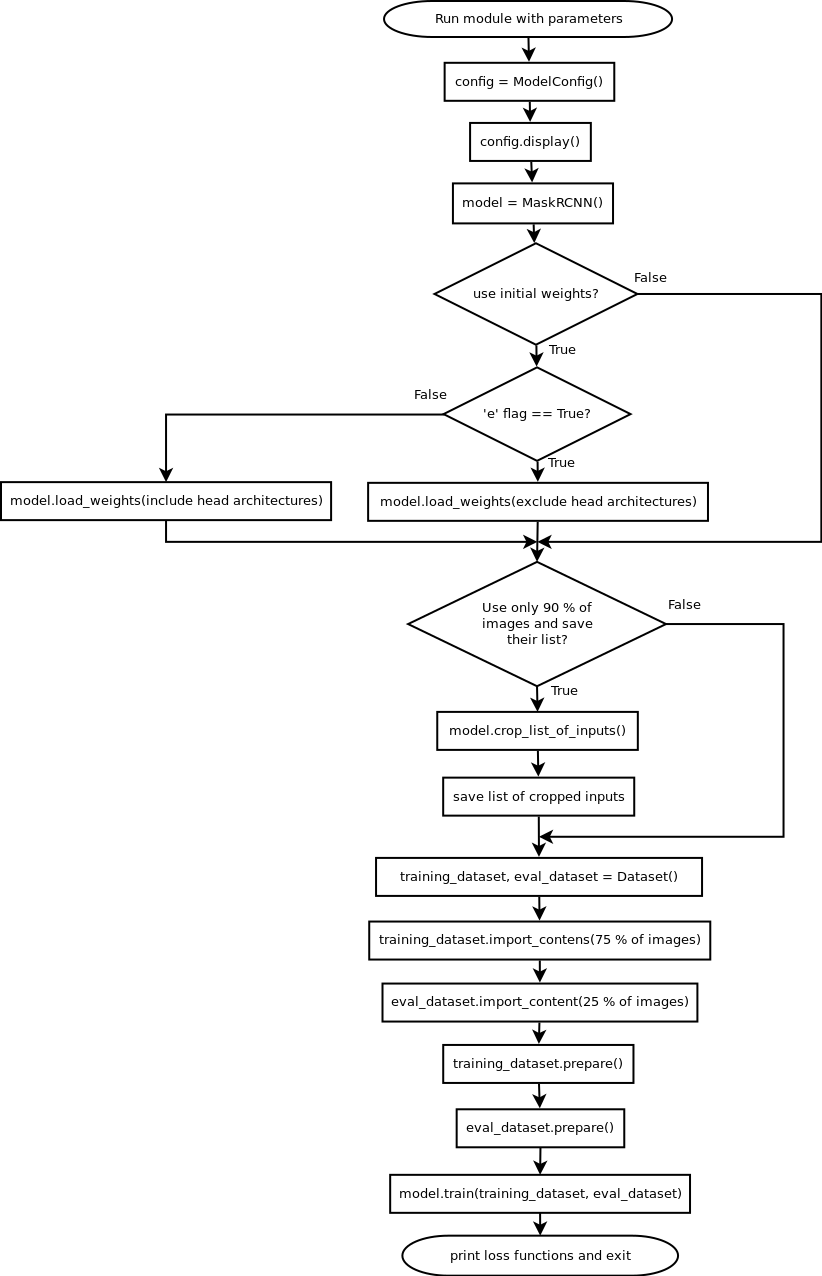
\includegraphics[width=0.95\linewidth]{./pictures/train_dia.png}
	\caption[ann.maskrcnn.train flowchart]{Flowchart of the ann.maskrcnn.train module}
      \label{fig:train}
\end{figure}

\begin{figure}[H]
   \centering
	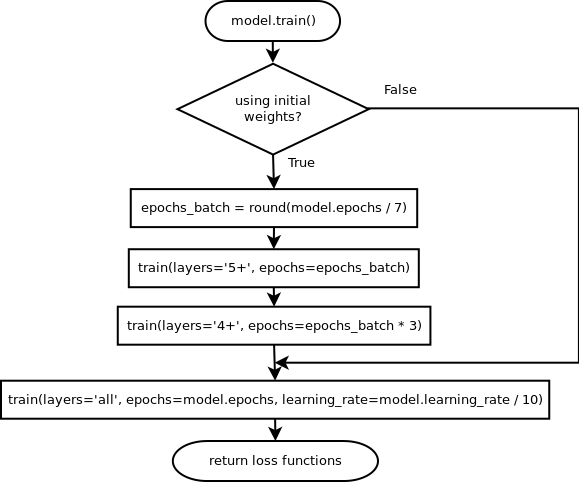
\includegraphics[width=\linewidth]{./pictures/training_dia.png}
	\caption[ann.maskrcnn.train training flowchart]{Flowchart of different training branches inside the ann.maskrcnn.train module}
      \label{fig:training}
\end{figure}

\verb|ann.maskrcnn.train| also contains its own manual, help and a graphical 
user interface (\zk{GUI}) to help a user's understanding of the module.

\section{ann.maskrcnn.detect}
\label{detect-module}

In case we have a trained model, either trained by us or provided by someone 
else, we can use it to detect features or objects in maps. Such maps have to be 
a georeferenced raster. The output from the module consists of a set of vector 
maps for each class. Although the model is to some extent scale-invariant, it is 
recommended to provide rasters in the same resolution as the ones used for the 
training. The detection is done in the \verb|ann.maskrcnn.detect| GRASS GIS 
module. The module is written in the file \verb|ann.maskrcnn.detect.py| and was 
written for the practical part of the thesis. Its workflow is with some 
simplifications illustrated in figure \ref{fig:detect}.

As in the \verb|ann.maskrcnn.train| module, the flowchart contains few 
already-mentioned functions and classes, specifically the \verb|ModelConfig| 
class from chapter \ref{config} and the \verb|MaskRCNN| class from chapter 
\ref{model-mrcnn}.

However, more unmentioned functions can be seen in the flowchart. Function
\verb|save_instances| saves masks of detected instances (by default they will be 
saved in the temporary GRASS folder, but the user is allowed to choose to keep 
them). These masks are rasters of the same size as the input images where mask 
pixels have the value of class ID and the rest are zeros. In case the original 
images were georeferenced internally (for example a \textit{GeoTIFF} format), 
the georeferencing is copied to saved rasters using \verb|GDAL|; otherwise (a 
flag \verb|-e| should be used), the function \verb|external_georeferencing| is 
called to copy georeferencing files to the directory with masks.

Rasters with masks are imported to GRASS GIS using the \verb|r.in.gdal| module, 
and then cropped and vectorized to get a separate vector map for each class. The~process
of cropping and vectorizing consists of a bunch of GRASS GIS modules and 
is illustrated in figure \ref{fig:vectorize}.

The illustrated process works only with detected classes (e.g. when no instance 
of sties was detected, the loop corresponding to this class will be skipped). 
The~term \verb|vector_map| used in the flowchart corresponds to the same string 
as the term \verb|raster_map|, but is used to emphasize the difference in the 
map type; it is also the reason why we can use \verb|v.patch| and 
\verb|g.remove| with \verb|vector_maps| - because we already have the list of 
raster maps. The motivation behind the inner loop in the~flowchart is a 
detection made on multiple rasters; classes from them are extracted and 
vectorized separately and then patched together for each class.

\begin{figure}[H]
   \centering
	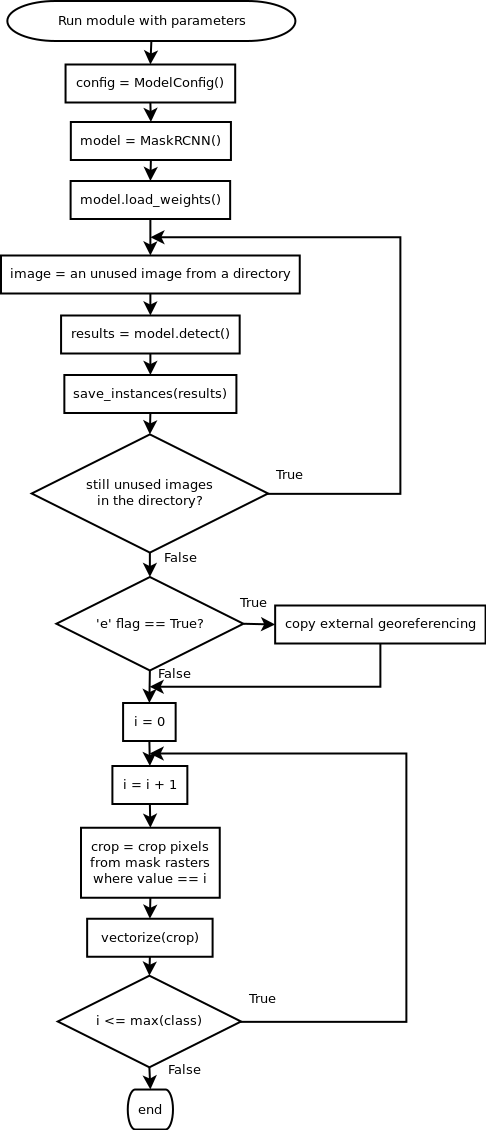
\includegraphics[width=0.6\linewidth]{./pictures/detect_dia.png}
	\caption[ann.maskrcnn.detect flowchart]{Flowchart of the ann.maskrcnn.detect module}
      \label{fig:detect}
\end{figure}

\begin{figure}[H]
   \centering
	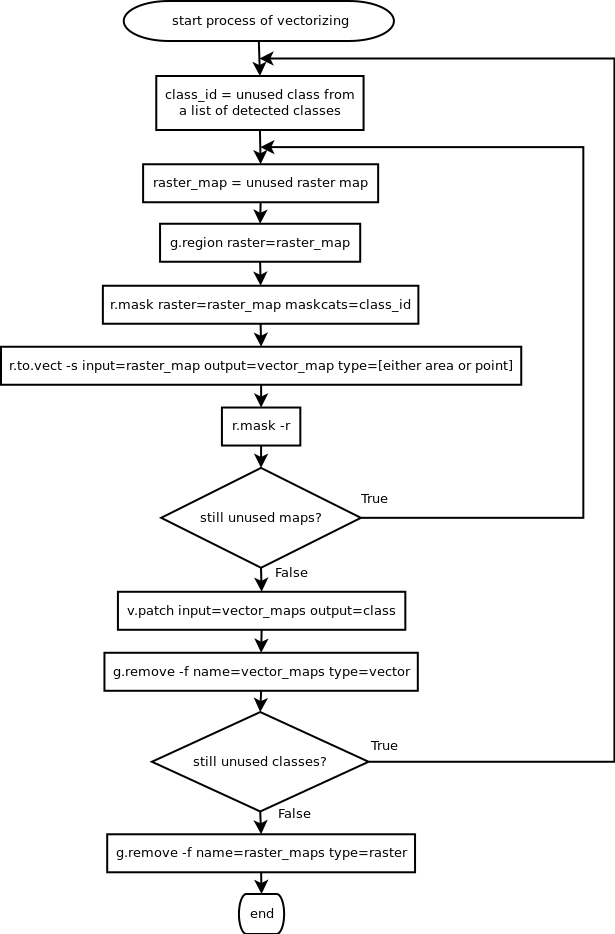
\includegraphics[width=0.95\linewidth]{./pictures/vectorize.png}
	\caption[vectorization in ann.maskrcnn.detect flowchart]{Flowchart of the vectorization and classes extraction in the ann.maskrcnn.detect module}
      \label{fig:vectorize}
\end{figure}

The output of \verb|ann.maskrcnn.detect| represents detected masks in a vector form. The output type can be either areas or points (corresponding to a centre of the mask).

\verb|ann.maskrcnn.detect| also contains its own manual, help and a \zk{GUI} to 
help a user's understanding of the module.

\section{GRASS GIS patch}
\label{grass-patch}

Although the support for Python 3 in GRASS GIS is a widely discussed topic and
although much effort has been done to for it, it is still not incompleted. This
lack is handled in modules, but there is still a problem in setting the GRASS
environment. Thus, a patch and a recompilation of GRASS are needed to allow the
user to set the environment right. The patch decode bytes-typed string into a
UTF-8-typed string and consists of the following \textit{diff}.

{\scriptsize
\begin{lstlisting}[basicstyle={\footnotesize\ttfamily},breaklines=True,
backgroundcolor = \color{light-gray}]
===================================================================
--- lib/python/script/core.py	(revision 72644)
+++ lib/python/script/core.py	(working copy)
@@ -746,7 +746,7 @@
         elif var.startswith(b'opt_'):
             options[var[4:]] = val
         elif var in [b'GRASS_OVERWRITE', b'GRASS_VERBOSE']:
-            os.environ[var] = val
+            os.environ[var.decode("utf-8")] = val.decode("utf-8")
         else:
             raise SyntaxError("invalid output from g.parser: %s" % line)
\end{lstlisting}}

\chapter{Conclusion}
\label{conclusion}

The goal of the~thesis was to find and implement a~suitable \zk{ANN} 
architecture into \zk{GRASS} \zk{GIS}. Because \zk{ANN}s and especially 
\zk{CNN}s are shaking with the~field of computer vision, many GRASS GIS users 
and developers were interested in implementation options into this system.

The first part of the~thesis was dedicated to a~theoretical background behind 
\zk{CNN}s. It is followed by their various applications in the~field of computer 
vision. 

The second part of the~thesis was dedicated to the implementation of Mask \zk{R-CNN} 
modules into GRASS GIS. It starts with a~brief introduction of some of the~used 
tools and follows with explanations of the~most important parts of the~code.

The research flows in the~background of the~theoretical part and is briefly 
summarized at the~beginning of the~chapter on the~implementation.

Developed modules are ready to use and as can be seen in appendices, I already 
made few tests. However, because the~training costs a~lot of time (at least few 
days on a~GPU machine, even weeks on a~machine without GPU), only a~limited 
amount of tests was made. Modules were proposed for testing also to other GRASS 
GIS developers and users and they found their results to be satisfying, 
sometimes even for data, where other methods of classification in GRASS GIS 
failed (a shadow over a~field, different colours, etc.).

Even though modules work, there are still some possible extensions and even some 
issues.

The biggest issue is in insufficient support for Python 3 in GRASS GIS. This 
issue is solved by a~patch attached as an e-attachment and should be solved in 
GRASS GIS during this year.

Possible extensions are:
\begin{itemize}
	\item Support more training data annotation structures. The~current state works with \verb|*.jpg| images and \verb|*.png| masks for each instance. The~next step could be a~JSON-based structure used in MS COCO\footnote{\url{http://cocodataset.org/\#format-data}}.
	\item Support training on images in GRASS GIS (using raster map as images, vector areas as masks).
	\item Support objects detection in images imported into GRASS GIS. The~current state works only with images outside GRASS GIS.
	\item Support more channels than three.
	\item Support more types of the~backbone architecture. Now only \zk{ResNet} 50 and \zk{ResNet} 101 are supported.
	\item Diversify head architecture types. The~current one is just very basic one.
\end{itemize}

The last thing worthy of mention is the~high gear of progress. After only six 
years of research in the~field of \zk{CNN}s, black is white and up is down. 
Everything has changed and results unbelievable six years back are standards 
nowadays. Almost every week, there is a~new architecture. Even during work on 
this project, many interesting architectures were proposed, to name a~few, 
\cite{masklab} or \cite{panoptic}.

Developed modules are the~first step of \zk{GRASS} \zk{GIS} in the~direction to 
neural networks. Many functions could be useful for developing more modules. It 
would be pleasant to start a~new trend and see more modules using \zk{CNN}s and 
sharing libraries. Unsupervised learning is an open call.


% vysázení seznamu zkratek

\begin{seznamzkratek}{ABCDE}

	\novazkratka{AI}
	      {AI}
	      {Artificial intelligence}
	\novazkratka{ANN}
	      {ANN}
	      {Artificial neural network}
	\novazkratka{CNN}
	      {CNN}
	      {Convolutional neural network}
	\novazkratka{DPM}
	      {DPM}
	      {Deformable part model}
	\novazkratka{FAIR}
	      {FAIR}
	      {Facebook AI research}
	\novazkratka{FC}
	      {FC}
	      {Fully connected}
	\novazkratka{FCN}
	      {FCN}
	      {Fully convolutional network}
	\novazkratka{FPN}
	      {FPN}
	      {Feature pyramid network}
	\novazkratka{GIS}
	      {GIS}
	      {Geographic information system}
	\novazkratka{GRASS}
	      {GRASS}
	      {Geographic resources analysis support system}
	\novazkratka{GUI}
	      {GUI}
	      {Graphical user interface}
	\novazkratka{ILSVRC}
	      {ILSVRC}
	      {ImageNet large scale visual recognition challenge}
	\novazkratka{IoU}
	      {IoU}
	      {Intersection over union}
	\novazkratka{mAP}
	      {mAP}
	      {Mean average precision}
	\novazkratka{R-CNN}
	      {R-CNN}
	      {Region-based convolutional neural network}
	\novazkratka{ReLU}
	      {ReLU}
	      {Rectified linear unit}
	\novazkratka{ResNet}
	      {ResNet}
	      {Residual network}
	\novazkratka{RNN}
	      {RNN}
	      {Recurrent neural network}
	\novazkratka{RoI}
	      {RoI}
	      {Region of interest}
	\novazkratka{RPN}
	      {RPN}
	      {Region proposal network}
	\novazkratka{SVM}
	      {SVM}
	      {Support vector machine}
	\novazkratka{VOC}
	      {VOC}
	      {Visual object classes}
	      
\end{seznamzkratek}

% literatura
\nocite{*}
\def\refname{References}
\bibliographystyle{mystyle}
\bibliography{literatura}


% začátek příloh
%\def\figurename{Figure}%
\prilohy

% vysázení seznamu příloh
\seznampriloh

% Vložení souboru s přílohami
\chapter{User manual}
\label{manual}

HTML pages in the style of common GRASS GIS user manuals were created. In this
chapter, they will be attached. Firstly, they will introduce Mask R-CNN tools
generally and then each module separately.

\section{Mask R-CNN tools}

\subsection*{DESCRIPTION}
Mask R-CNN tools allow the user to train his own model and use it for a 
detection of objects, or to use a model provided by someone else. It can be seen 
as a supervised classification using convolutional neural networks.

The training is done using module \emph{ann.maskrcnn.train}. The user feeds the 
module with training data consisting of images and masks for each instance of 
intended classes, and gets a model. For difficult tasks and when not using a 
pretrained model, the training may take even weeks; in case of a good pretrained 
model and powerful PC with GPU support, the training could get good results 
after 1 day and even less.

When the user has a model, it can be used for the detection. 
\emph{ann.maskrcnn.detect} detects classes learned during the training and 
extracts from given images vectors corresponding to detected objects. Objects 
can be extracted either as areas or points. 

\subsection*{MODULES}
\emph{ann.maskrcnn.train},\emph{ }\emph{ann.maskrcnn.detect}\emph{ }

\clearpage

\section{ann.maskrcnn.train}

\subsection*{NAME}

\textbf{ann.maskrcnn.train -} Train your Mask R-CNN network.

\subsection*{SYNOPSIS}

\begin{flushleft}
\textbf{ann.maskrcnn.train} 

\textbf{ann.maskrcnn.train -{}-help}

\textbf{ann.maskrcnn.train} [\textbf{-esbn}] \textbf{training\_dataset}=name [\textbf{model}=string] \tab\ \textbf{classes}=string[,string,...] \textbf{logs}=name \textbf{name}=string [\textbf{epochs}=value] \tab\ [\textbf{steps\_per\_epoch}=value] [\textbf{rois\_per\_image}=value] \tab\ [\textbf{images\_per\_gpu}=value] [\textbf{gpu\_count}=value] \tab\ [\textbf{mini\_mask\_size}=value[,value,...]] [\textbf{validation\_steps}=value] \tab\ [\textbf{images\_min\_dim}=value] [\textbf{images\_max\_dim}=value] \tab\ [\textbf{backbone}=string] [\textbf{-{}-overwrite}] [\textbf{-{}-help}] [\textbf{-{}-verbose}] [\textbf{-{}-quiet}] [\textbf{-{}-ui}]
\end{flushleft}

\subsubsection*{Flags:}
\begin{flushleft}
  \textbf{-e}
  
  \tab Pretrained weights were trained on another classes / resolution / sizes
  
  \textbf{-s}
  
  \tab Do not use 10 \% of images and save their list to logs dir
  
  \textbf{-b}
  
  \tab Train also batch normalization layers (not recommended for small batches)

  \textbf{-n}
  
  \tab No resizing or padding of images (images must be of the same size)
  
  \textbf{-{}-overwrite}
  
  \tab Allow output files to overwrite existing files
  
  \textbf{-{}-help}
  
  \tab Print usage summary
  
  \textbf{-{}-verbose}
  
  \tab Verbose module output
  
  \textbf{-{}-quiet}
  
  \tab Quiet module output
  
  \textbf{-{}-ui}
  
  \tab Force launching GUI dialog
\end{flushleft}

\subsubsection*{Parameters:}

\begin{flushleft}
\textbf{training\_dataset}=name \textbf{[required]}

\tab Path to the dataset with images and masks

\textbf{model}=string

\tab Path to the .h5 file to use as initial values

\tab Keep empty to train from a scratch

\textbf{classes}=string[,string,...] \textbf{[required]}
           
\tab Names of classes separated with ","

\textbf{logs}=name \textbf{[required]}

\tab Path to the directory in which will be models saved

\textbf{name}=string \textbf{[required]}

\tab Name for output models

\textbf{epochs}=value

\tab Number of epochs

\tab default: 200

\textbf{steps\_per\_epoch}=value

\tab Steps per each epoch

\tab default: 3000

\textbf{rois\_per\_image}=value

\tab How many ROIs train per image

\tab default: 64

\textbf{images\_per\_gpu}=value

\tab Number of images per GPU

\tab Bigger number means faster training but needs a bigger GPU

\tab default: 1

\textbf{gpu\_count}=value

\tab Number of GPUs to be used

\tab default: 1

\textbf{mini\_mask\_size}=value[,value,...]

\tab Size of mini mask separated with ","

\tab To use full sized masks, keep empty.

\tab Mini mask saves memory at the expense of precision

\textbf{validation\_steps}=value

\tab Number of validation steps

\tab Bigger number means more accurate estimation of the model precision

\tab default: 100

\textbf{images\_min\_dim}=value

\tab Minimum length of images sides

\tab Images will be resized to have their shortest side at least of this value

\tab Has to be a multiple of 64

\tab default: 256

\textbf{images\_max\_dim}=value

\tab Maximum length of images sides

\tab Images will be resized to have their longest side of this value

\tab Has to be a multiple of 64

\tab default: 1280

\textbf{backbone}=string

\tab Backbone architecture

\tab options: resnet50, resnet101

\tab default: resnet101
\end{flushleft}

\subsection*{DESCRIPTION}
\textstyleEmphasis{ann.maskrcnn.train} allows user to train a Mask R-CNN model
on his own dataset. The dataset has to be prepared in a predefined structure. 

\subsubsection*{DATASET STRUCTURE}
Training dataset should be in the following structure: 

\liststyleLi
\begin{itemize}
\item dataset-directory
\begin{itemize}
\item imagenumber 

\begin{itemize}
\item imagenumber.jpg (training image) 
\item imagenumber-class1-number.png (mask for one instance of class1) 
\item imagenumber-class1-number.png (mask for another instance of class1) 
\item ... 
\end{itemize}
\item imagenumber2 

\begin{itemize}
\item imagenumber2.jpg 
\item imagenumber2-class1-number.png (mask for one instance of class1) 
\item imagenumber2-class2-number.png (mask for another class instance) 
\item ... 
\end{itemize}
\end{itemize}
\end{itemize}

The described structure of directories is required. Pictures must be *.jpg files
with 3 channels (for example RGB), masks must be *.png files consisting of
numbers between 1 and 255 (object instance) and 0s (elsewhere). A mask file for
each instance of object should be provided separately distinguished by the
suffix number. 

\subsection*{NOTES}
If you are using initial weights (the \textstyleEmphasis{model} parameter),
epochs are divided into three segments. Firstly training layers 5+, then
fine-tuning layers 4+ and the last segment is fine-tuning the whole
architecture. Ending number of epoch is shown for your segment, not for the
whole training. 

The usage of the \textstyleEmphasis{{}-b} flag will result in an activation of
batch normalization layers training. By default, this option is set to False,
as it is not recommended to train them when using just small batches (batch is
defined by the \textstyleEmphasis{images\_per\_gpu} parameter). 

If the dataset consists of images of the same size, the user may use the
\textstyleEmphasis{{}-n} flag to avoid resizing or padding of images. When the
flag is not used, images are resized to have their longer side equal to the
value of the \textstyleEmphasis{images\_max\_dim} parameter and the shorter
side longer or equal to the value of the \textstyleEmphasis{images\_min\_dim}
parameter and zero-padded to be of shape \verb|images\_max\_dim| $\times$
\verb|images\_max\_dim|. It results in the fact that even images of different
sizes may be used. 

After each epoch, the current model is saved. It allows the user to stop the~training
when he feels satisfied with loss functions. It also allow the user to
test models even during the training (and, again, stop it even before the last
epoch). 

\subsection*{EXAMPLES}
Dataset for examples: 

\liststyleLii
\begin{itemize}
\item crops 

\begin{itemize}
\item 000000 

\begin{itemize}
\item 000000.jpg 
\item 000000-corn-0.png 
\item 000000-corn-1.png 
\item ... 
\end{itemize}
\item 000001 

\begin{itemize}
\item 000001.jpg 
\item 000001-corn-0.png 
\item 000001-rice-0.png 
\item ... 
\end{itemize}
\end{itemize}
\end{itemize}

\subsubsection*{Training from scratch}
\begin{lstlisting}[breaklines=true]
ann.maskrcnn.train training_dataset=/home/user/Documents/crops classes=corn,rice logs=/home/user/Documents/logs name=crops
\end{lstlisting}

After default number of epochs we will get a model where the first class is
trained to detect corn fields and the second one to detect rice fields. 

If we use the command with reversed classes order, we will get a model where the
first class is trained to detect rice fields and the second one to detect corn
fields:

\begin{lstlisting}[breaklines=true]
ann.maskrcnn.train training_dataset=/home/user/Documents/crops classes=rice,corn logs=/home/user/Documents/logs name=crops
\end{lstlisting}

The name of the model does not have to be the same as the dataset folder, but
should be referring to the task of the dataset. A good name for this one
(referring also to the order of classes) could be also this one: 

\begin{lstlisting}[breaklines=true]
ann.maskrcnn.train training_dataset=/home/user/Documents/crops classes=rice,corn logs=/home/user/Documents/logs name=rice_corn
\end{lstlisting}

\subsubsection*{Training from a pretrained model}
We can use a pretrained model to make our training faster. It is necessary for
the~model to be trained on the same channels and similar features, but it does
not have to be the same ones (e.g. model trained on swimming pools in maps can
be used for a training on buildings in maps). 

A model trained on different classes (use \textstyleEmphasis{{}-e} flag to
exclude head weights):

\begin{lstlisting}[breaklines=true]
ann.maskrcnn.train training_dataset=/home/user/Documents/crops classes=corn,rice logs=/home/user/Documents/logs name=crops model=/home/user/Documents/models/buildings.h5 -e
\end{lstlisting}

A model trained on the same classes:

\begin{lstlisting}[breaklines=true]
ann.maskrcnn.train training_dataset=/home/user/Documents/crops classes=corn,rice logs=/home/user/Documents/logs name=crops model=/home/user/Documents/models/corn_rice.h5
\end{lstlisting}

\subsubsection*{Fine-tuning a model}
It is also possible to stop your training and then continue. To continue in the
training, just use the last saved epoch as a pretrained model:

\begin{lstlisting}[breaklines=true]
ann.maskrcnn.train training_dataset=/home/user/Documents/crops classes=corn,rice logs=/home/user/Documents/logs name=crops model=/home/user/Documents/models/mask_rcnn_crops_0005.h5
\end{lstlisting}

\clearpage

\section{ann.maskrcnn.detect}

\subsection*{NAME}

\textbf{ann.maskrcnn.detect -} Detect features in images using a Mask R-CNN model.

\subsection*{SYNOPSIS}

\begin{flushleft}
\textbf{ann.maskrcnn.detect} 

\textbf{ann.maskrcnn.detect -{}-help}

\textbf{ann.maskrcnn.detect} [\textbf{-esbn}] \textbf{images\_directory}=name \tab\ \textbf{images\_format}=string \textbf{model}=string \textbf{classes}=string[,string,...] \tab\ [\textbf{masks\_output}=name] [\textbf{output\_type}=string] [\textbf{-{}-overwrite}] [\textbf{-{}-help}] \tab\ [\textbf{-{}-verbose}] [\textbf{-{}-quiet}] [\textbf{-{}-ui}]
\end{flushleft}

\subsubsection*{Flags:}
\begin{flushleft}
  \textbf{-e}
  
  \tab External georeferencing in the images folder
  
  \textbf{-{}-overwrite}
  
  \tab Allow output files to overwrite existing files
  
  \textbf{-{}-help}
  
  \tab Print usage summary
  
  \textbf{-{}-verbose}
  
  \tab Verbose module output
  
  \textbf{-{}-quiet}
  
  \tab Quiet module output
  
  \textbf{-{}-ui}
  
  \tab Force launching GUI dialog
\end{flushleft}

\subsubsection*{Parameters:}

\begin{flushleft}
\textbf{images\_directory}=name \textbf{[required]}

\tab Path to a directory with images to detect

\textbf{images\_format}=string \textbf{[required]}

\tab Format suffix of images

\textbf{model}=string \textbf{[required]}

\tab Path to the .h5 file containing the model

\textbf{classes}=string[,string,...] \textbf{[required]}
           
\tab Names of classes separated with ","

\textbf{masks\_output}=name

\tab Directory where masks will be saved

\textbf{output\_type}=string

\tab Type of output

\tab options:area, point

\tab default: area
\end{flushleft}

\subsection*{DESCRIPTION}
\textstyleEmphasis{ann.maskrcnn.detect} allows user to use a Mask R-CNN model to
detect features in georeferenced files and extract them either as areas or
points. The module creates a~separate map for each class. 

\subsection*{NOTES}
The detection may be used for multiple files. However, all files for the
detection must be in one directory specified in the
\textstyleEmphasis{images\_directory} parameter. Even when using only one
image, the module finds it through this parameter. 

When detecting, you can use new names of classes. Classes in the model are not
referenced by their name, but by their order. It means that if the model was
trained with classes \textstyleEmphasis{corn,rice} and you use
\textstyleEmphasis{ann.maskrcnn.detect} with classes
\textstyleEmphasis{zea,oryza}, zea areas will present areas detected as corn
and oryza areas will present areas detected as rice. 

If the file is georeferenced externally (by a worldfile or an
\textstyleEmphasis{.aux.xml} file), please use \textstyleEmphasis{{}-e} flag. 

\subsection*{EXAMPLES}
\subsubsection*{Detect buildings and lakes and import them as areas}
In case the georeferencing is internal (GeoTIFF): 

\begin{lstlisting}[breaklines=true]
ann.maskrcnn.detect images_directory=/home/user/Documents/georeferenced_images classes=buildings,lakes model=/home/user/Documents/logs/mask_rcnn_building_lakes_0100.h5 images_format=tif
\end{lstlisting}

\ \linebreak In case the georeferencing is external: 

\begin{lstlisting}[breaklines=true]
ann.maskrcnn.detect images_directory=/home/user/Documents/georeferenced_images classes=buildings,lakes model=/home/user/Documents/logs/mask_rcnn_building_lakes_0100.h5 images_format=png -e
\end{lstlisting}

\subsubsection*{Detect cottages and plattenbaus and import them as points}
\begin{lstlisting}[breaklines=true]
ann.maskrcnn.detect images_directory=/home/user/Documents/georeferenced_images classes=cottages,plattenbaus model=/home/user/Documents/logs/mask_rcnn_houses_0100.h5 images_format=tif output_type=point
\end{lstlisting}


% konec dokumentu
\end{document}
